\documentclass[11pt]{article}
\pdftrailerid{}
\pdfinfoomitdate=1
\pdfsuppressptexinfo=-1
\input{glyphtounicode}
\pdfglyphtounicode{mapsto}{007C}
\pdfglyphtounicode{parenleftbig}{0028}
\pdfglyphtounicode{parenrightbig}{0029}
\pdfglyphtounicode{bracketleftbig}{005B}
\pdfglyphtounicode{bracketrightbig}{005D}
\pdfglyphtounicode{vextendsingle}{007C}
\pdfglyphtounicode{vextenddouble}{2225}
\pdfglyphtounicode{parenleftBig}{0028}
\pdfglyphtounicode{parenrightBig}{0029}
\pdfglyphtounicode{parenleftbigg}{0028}
\pdfglyphtounicode{parenrightbigg}{0029}
\pdfglyphtounicode{bracketleftbigg}{005B}
\pdfglyphtounicode{bracketrightbigg}{005D}
\pdfglyphtounicode{parenleftBigg}{0028}
\pdfglyphtounicode{parenrightBigg}{0029}
\pdfglyphtounicode{parenlefttp}{239B}
\pdfglyphtounicode{parenrighttp}{239E}
\pdfglyphtounicode{bracketlefttp}{23A1}
\pdfglyphtounicode{bracketrighttp}{23A4}
\pdfglyphtounicode{bracketleftbt}{23A3}
\pdfglyphtounicode{bracketrightbt}{23A6}
\pdfglyphtounicode{bracelefttp}{23A7}
\pdfglyphtounicode{braceleftbt}{23A9}
\pdfglyphtounicode{braceleftmid}{23A8}
\pdfglyphtounicode{braceex}{23AA}
\pdfglyphtounicode{parenleftbt}{239D}
\pdfglyphtounicode{parenrightbt}{23A0}
\pdfglyphtounicode{angbracketleftBig}{27E8}
\pdfglyphtounicode{angbracketrightBig}{27E9}
\pdfglyphtounicode{summationtext}{2211}
\pdfglyphtounicode{producttext}{220F}
\pdfglyphtounicode{integraltext}{222B}
\pdfglyphtounicode{summationdisplay}{2211}
\pdfglyphtounicode{productdisplay}{220F}
\pdfglyphtounicode{integraldisplay}{222B}
\pdfglyphtounicode{hatwide}{0302}
\pdfglyphtounicode{bracketleftBig}{005B}
\pdfglyphtounicode{bracketrightBig}{005D}
\pdfgentounicode=1

\usepackage[T1]{fontenc}
\usepackage{lmodern}
\usepackage[margin=1.05in]{geometry}
\usepackage{amsmath,amssymb,amsthm,mathtools,mathrsfs}
\usepackage[expansion=false]{microtype}
\usepackage{enumitem}
\usepackage{tikz}
\usepackage{xcolor}
\PassOptionsToPackage{hyphens}{url}
\usepackage[colorlinks=true,linkcolor=blue!50!black,citecolor=blue!50!black,urlcolor=blue!50!black]{hyperref}
\usepackage[nameinlink,capitalise,noabbrev]{cleveref}
\hypersetup{bookmarksdepth=2,
 pdftitle={The M\'ezard--Parisi formula for diluted spin glasses},
 pdfauthor={OpenAI}}
\numberwithin{equation}{section}
\newtheorem{theorem}{Theorem}[section]
\newtheorem{proposition}[theorem]{Proposition}
\newtheorem{lemma}[theorem]{Lemma}
\newtheorem{corollary}[theorem]{Corollary}
\theoremstyle{definition}
\newtheorem{definition}[theorem]{Definition}
\theoremstyle{remark}
\newtheorem{remark}[theorem]{Remark}
\newcommand{\E}{\mathbb E}
\renewcommand{\P}{\mathbb P}
\newcommand{\R}{\mathbb R}
\newcommand{\N}{\mathbb N}
\newcommand{\cB}{\mathcal B}
\newcommand{\cF}{\mathcal F}
\newcommand{\cT}{\mathcal T}
\newcommand{\eps}{\varepsilon}
\newcommand{\dd}{\,\mathrm d}
\newcommand{\norm}[1]{\lVert#1\rVert}
\newcommand{\abs}[1]{\lvert#1\rvert}
\newcommand{\angles}[1]{\langle#1\rangle}
\DeclareMathOperator{\Var}{Var}
\DeclareMathOperator{\Cov}{Cov}
\DeclareMathOperator{\arctanh}{arctanh}
\DeclareMathOperator{\Pois}{Poisson}
\DeclareMathOperator{\supp}{supp}
\setlist{topsep=4pt,itemsep=2pt}
\setcounter{tocdepth}{1}
\setlength{\emergencystretch}{2em}
\title{The M\'ezard--Parisi formula for diluted spin glasses}
\author{OpenAI}
\date{September 23, 2026}
\begin{document}
\maketitle
\begin{abstract}
We prove the M\'ezard--Parisi hierarchical cavity formula for diluted
even-arity Ising models in the Panchenko--Talagrand class. This resolves
the variational equality conjecture for that class: the limiting pressure
equals the infimum of the trial functional over all finite hierarchy depths
and trial laws. Only first moments of the interaction and external field
are required.
\end{abstract}
\section{Introduction}

A diluted spin glass has a finite mean number of interactions per spin.
Its local environment remains random as the system grows, and the cavity
method describes that environment through a distribution of local fields.
When many competing states contribute to the partition function, the
proposed order parameter is a hierarchy of distributions of these fields.
The thermodynamic question is whether this hierarchy determines the
limiting expected log partition function per spin. We call this quantity
\emph{pressure}. At inverse temperature $\beta$, the usual physical free
energy per spin is its negative divided by $\beta$.

The Viana--Bray model is a classical diluted two-spin
model~\cite{VB85}. M\'ezard and Parisi~\cite{MP01} developed the
hierarchical cavity picture for the fixed-connectivity Bethe-lattice
spin glass, with an explicit one-step replica-symmetry-breaking
functional. Franz and Leone~\cite{FL03} adapted Guerra's
interpolation method~\cite{Guerra03} to diluted systems and obtained
replica-symmetric and one-step pressure bounds for even-arity models.
Panchenko and
Talagrand~\cite{PT04} then proved the arbitrary finite-level
hierarchical upper bounds considered here.

We prove that the infimum of these bounds is the limiting pressure.
This resolves the equality conjecture stated immediately after
Theorem~4 of Panchenko--Talagrand~\cite{PT04}, for their Poisson,
even-arity Ising model class with factorized interactions and the
specified positivity condition. Only first moments of the interaction
and external field are required. The result includes the Viana--Bray
model, diluted even-spin models with symmetric couplings, and soft
random even-$K$ SAT at every positive temperature. The exact model and
trial functional are defined in \cref{model:section}; the named models
and their expected ground-state limits are treated in
\cref{models:section}.

An exact variational description and reduction to a prescribed
trial class are distinct problems. The cavity variational principle of
Aizenman, Sims and Starr~\cite{ASS03} for the Sherrington--Kirkpatrick model
has a Viana--Bray counterpart in De Sanctis's formulation over random
multioverlap structures~\cite{DeSanctis04}. Panchenko's
spin-distribution approach~\cite[Theorems~1--2]{Pan13} gives an exact
variational formula over invariant exchangeable spin distributions.
Under their positivity condition, Coja-Oghlan and
Perkins~\cite{COP19} obtain an invariant-kernel variational formula
for random regular factor graphs. These results
use different descriptions of the state from the finite hierarchy of
message laws optimized here. The additional task is to recover the
specific hierarchical cavity functional without losing the pressure.

Panchenko~\cite[Theorem~2]{Pan16} established a hierarchical
single-site representation for finite-RSB asymptotic Gibbs measures of
suitably modified models; approximation of general states by that class
remains a separate step. Biswas, Chen and
Sen~\cite[Theorem~1.1 and Proposition~1.4]{BCS25} obtain exact
replica-symmetric pressure formulas in high-temperature and critical or
subcritical regimes for compact real spin spaces under moment and regularity
assumptions. For the zero-field Ising spin glass with Rademacher couplings
on random regular graphs, Concetti~\cite[Theorem~1.3]{Concetti25}
gives a full-replica-symmetry-breaking pressure bound no larger than each
optimized finite-level bound; equality with that functional is
conjectural in that work. The result here
identifies the finite-depth Panchenko--Talagrand infimum at arbitrary
density in its stated interaction class.

The main obstacle is the distribution of spins seen across several
replicas, that is, several samples from the same Gibbs system. The
probability of each replica-spin pattern depends on products of every
subset of those spins. The spatial average of such a product is a
\emph{multioverlap}; pair overlaps alone do not determine all these
patterns. This is the information isolated by the spin-distribution
approach~\cite{Pan13}. To compare a cavity insertion with independent
hierarchical messages, we must control all finite multioverlaps before
redrawing the message roots independently.

We work with finite auxiliary hierarchies before taking the
thermodynamic limit. Their branching is part of the construction;
no ultrametric organization of the physical Gibbs states is assumed.
Bounded perturbations yield identities for
prescribed replica branching patterns. Delaying each branching depth
by one level permits an induction that concentrates multioverlaps
\emph{on average over branching depths}. The cavity insertion itself
has an expansion averaging over finite trees, so this averaged control
is sufficient. The system size tends to infinity at each fixed depth;
only then does the depth increase. The proof strategy following
\cref{main:theorem} explains how the finite-tree calculus, concentration
and independent-message comparison fit together.

\section{The model and the variational principle}\label{model:section}

Fix an even integer $p\ge2$ and $\alpha>0$. Let $\theta$ be a random real
function on $\{-1,1\}^p$ and let $h$ be a real random variable. Write
$B(\theta)=\max_s\abs{\theta(s)}$ and assume
\begin{equation}\label{model:integrability}
 \E B(\theta)+\E\abs h<\infty.
\end{equation}
For independent $M_N\sim\Pois(\alpha N)$, independent copies $\theta_k$ of
$\theta$, independent copies $h_i$ of $h$, and independent uniform indices
$i_{\ell,k}\in[N]=\{1,\ldots,N\}$, set
\begin{equation}\label{model:hamiltonian}
 \begin{gathered}
 -H_N(\sigma)=\sum_{k=1}^{M_N}
 \theta_k(\sigma_{i_{1,k}},\ldots,\sigma_{i_{p,k}})
 +\sum_{i=1}^N h_i\sigma_i,\\
 Z_N=\sum_{\sigma\in\{-1,1\}^N}e^{-H_N(\sigma)},
 \qquad F_N=\frac1N\E\log Z_N.
 \end{gathered}
\end{equation}
All families in this definition are mutually independent. In particular,
indices are sampled with replacement. The model parameters and disorder
laws are fixed as $N$ varies.

The interaction hypotheses are the existence of a representation
\begin{equation}\label{model:factorization}
 e^{\theta(s_1,\ldots,s_p)}
 =a\left(1+b\prod_{\ell=1}^p f_\ell(s_\ell)\right),
 \qquad
 \abs{b\prod_{\ell=1}^p f_\ell(s_\ell)}<1\quad\text{a.s.},
\end{equation}
for every spin tuple, where $a>0$ and $b$ are real random variables,
the $f_\ell:\{-1,1\}\to\R$ are independent copies of one random
function, $b$ is independent of them, and
\begin{equation}\label{model:positivity}
 \E[(-b)^n]\ge0\qquad(n\ge1).
\end{equation}
The expectations in \eqref{model:positivity} are interpreted as finite real
expectations. This is automatic in the nondegenerate case: independence
and the strict product bound force $b$ and $\max_s|f_1(s)|$ to be
essentially bounded, as shown in \cref{upper:bound}. If the product term
vanishes identically, the interaction is spin independent and one may
take $b=0$. The multiplier $a$ may depend on all the other variables in
the representation; no separate integrability of $\log a$ is assumed.

\subsection{The hierarchical cavity functional}

We give the power-mean form of the Panchenko--Talagrand functional
\cite[Section~5]{PT04}. A message $x$ specifies a probability distribution
on one spin. The site term inserts a new spin with its incident
interactions; the edge term corrects for interactions counted in that
insertion.

For $x\in\R$ let $q_x(s)=e^{xs}/(2\cosh x)$. Define
\begin{align}
 C_\theta(x_1,\ldots,x_p)
 &=\sum_{s\in\{-1,1\}^p}e^{\theta(s)}\prod_{\ell=1}^p q_{x_\ell}(s_\ell),
 \label{model:edge}\\
 U_\theta(x_1,\ldots,x_{p-1};\eps)
 &=\log\sum_{s\in\{-1,1\}^{p-1}}
 e^{\theta(s_1,\ldots,s_{p-1},\eps)}
 \prod_{\ell=1}^{p-1}q_{x_\ell}(s_\ell).
 \label{model:site-message}
\end{align}
Both $\abs{\log C_\theta}$ and $\abs{U_\theta}$ are bounded by $B(\theta)$,
uniformly in the messages.

Write $\mathcal P(E)$ for the Borel probability measures on $E$.
Let $\mathcal M_1=\mathcal P(\R)$ and
$\mathcal M_{j+1}=\mathcal P(\mathcal M_j)$, equipped with the topology of weak convergence and its Borel sigma-field. Fix $r\ge1$, $\zeta\in\mathcal M_{r+1}$, and
$0<m_1<\cdots<m_r<1$. For each message label $\omega$ independently, draw
\begin{equation}\label{model:chain}
 \eta_0^\omega\sim\zeta,\qquad
 \eta_{d+1}^\omega\mid\eta_d^\omega\sim\eta_d^\omega\ (0\le d\le r-2),
 \qquad x^\omega\mid\eta_{r-1}^\omega\sim\eta_{r-1}^\omega.
\end{equation}
At $r=1$, this means that each label first draws a random probability
measure $\eta_0$ with law $\zeta$, then draws $x$ with law $\eta_0$.
Higher levels repeat this sampling of measures. All these variables are
independent of the physical disorder. Use different
labels for $x_1,\ldots,x_p$ and for $x_\ell^j$, $j\ge1$, $1\le\ell<p$.
Take independent $k\sim\Pois(\alpha p)$, $\theta,\theta_1,\ldots$, and $h$,
and put
\begin{align}
 V_{\rm s}&=\frac12\sum_{\eps=\pm1}
 \exp\left(h\eps+\sum_{j=1}^k
 U_{\theta_j}(x_1^j,\ldots,x_{p-1}^j;\eps)\right),\label{model:vs}\\
 V_{\rm e}&=C_\theta(x_1,\ldots,x_p).\label{model:ve}
\end{align}
For $0\le d<r$, let $\mathscr F_d$ be generated by all the physical disorder in these
expressions and all $\eta_j^\omega$, $0\le j\le d$. Set
\begin{equation}\label{model:power-means}
 T_rV=V,\qquad
 T_dV=\left(\E[(T_{d+1}V)^{m_{d+1}}\mid\mathscr F_d]\right)^{1/m_{d+1}}
 \quad(d=r-1,\ldots,0).
\end{equation}
Only auxiliary messages are integrated in these conditional expectations.
For example, at depth one,
$T_0V=(\E_x[V^{m_1}\mid\boldsymbol\eta_0])^{1/m_1}$.
At depth two, each label draws
$\eta_0\sim\zeta$, then $\eta_1\mid\eta_0\sim\eta_0$, and then
$x\mid\eta_1\sim\eta_1$, and
\[
 T_0V=\left(\E_{\boldsymbol\eta_1}
   \left[\left(\E_{\boldsymbol x}
      [V^{m_2}\mid\boldsymbol\eta_1]\right)^{m_1/m_2}
      \,\middle|\,\boldsymbol\eta_0\right]\right)^{1/m_1}.
\]
Here bold symbols collect all message labels in $V$; physical disorder is
held fixed throughout, including in the two abbreviated displays.
Define
\begin{equation}\label{model:functional}
 \cB_r(\zeta,\mathbf m)
 =\log2+\E\log T_0V_{\rm s}
 -\alpha(p-1)\E\log T_0V_{\rm e},
 \qquad \Phi_r=\inf_{\zeta,\,\mathbf m}\cB_r(\zeta,\mathbf m).
\end{equation}
At $r=0$, the messages are independent with common law
$\zeta\in\mathcal P(\R)$ and the operators $T_d$ are omitted; this defines
$\cB_0(\zeta)$ and $\Phi_0$.

The quantities in \eqref{model:functional} are finite without any moment
assumption on the trial messages. Indeed, the power-mean operators preserve
pointwise multiplicative bounds, and
\begin{equation}\label{model:trial-bounds}
 \abs{\log T_0V_{\rm s}}\le\abs h+\sum_{j=1}^k B(\theta_j),
 \qquad \abs{\log T_0V_{\rm e}}\le B(\theta).
\end{equation}

\begin{theorem}\label{main:theorem}
Under \eqref{model:integrability}--\eqref{model:positivity}, the thermodynamic
limit exists and
\begin{equation}\label{main:formula}
 \lim_{N\to\infty}F_N=\inf_{r\ge0}\Phi_r.
\end{equation}
\end{theorem}

The right side is an infimum over finite hierarchies. The theorem does not
assume that a trial law attains it or that a limiting infinite-depth
Gibbs state has been constructed.

\subsection{Proof strategy}

The interpolation upper bound holds at every system size and every
finite depth. We reproduce it in \cref{upper:section}, including a
normalization that avoids assuming integrability of the multiplier
$\log a$. The lower bound has four steps.

\begin{enumerate}[label=\textup{\arabic*.},leftmargin=*]
\item \emph{Select a cavity reservoir.}
A reservoir is a common Gibbs system on $N$ spins used to compare
systems of sizes $N$ and $N+1$.
For bounded interaction and field laws, add bounded Poisson perturbations whose
number is sublinear in the system size. Their effect on the pressure
vanishes. At each fixed hierarchy depth, select system sizes and
deterministic perturbation parameters for which the difference between
successive expected logarithms after the auxiliary power-mean recursion
is at most an arbitrarily small error above the original pressure liminf. The same choices give concentration of every
perturbation score (\cref{cavity:section,pert:selection}).

\item \emph{Prescribe branching patterns.}
An elementary calculus for finite probability trees expands insertions
into signed sums over added replica paths. Independent marks select any
prescribed branching pattern. Score concentration then gives identities
for these signed sums (\cref{tree:section,pert:tree-identity}).

\item \emph{Concentrate all multioverlaps.}
Move each internal branching depth of a target tree one step later.
The first fresh split at each new depth supplies the same small factor
as the normalizing coefficient. A relative bound on the sum of absolute
coefficients preserves control of errors after division. Conditional
covariance then decays by induction on the number of replicas.
A second identity concentrates the remaining conditional mean
(\cref{decor:section}).

\item \emph{Recover independent cavity messages.}
Encode a uniformly chosen reservoir site's entire finite hierarchy by
successive conditional laws. Multioverlap concentration permits different
site labels to be replaced by independent copies of this process in
the cavity insertion. This yields an admissible trial value close to
the selected increment (\cref{comp:section}).
\end{enumerate}

The estimates in Step~3 are averages over separated interior branching
depths. The insertion expansion assigns vanishing probability to the
exceptional trees, so these averages are sufficient for Step~4. No
uniform concentration in the depth is needed. The resulting lower bound
holds for every bounded interaction law invariant under permutations of
its inputs, without factorization or positivity. Finally, normalization
and estimates uniform over all trial laws remove boundedness and give
\cref{main:theorem} under the stated first moment assumption
(\cref{reduction:section}).

\section{Calculus on finite trees}\label{tree:section}

A power-mean insertion admits two expansions.  The logarithmic expansion
will compare pressures; an expansion with one canceled replica factor
will extract the perturbation identities.  Both follow from one
differentiation rule on trees.  We also bound their coefficients and the
probability of exceptional branching depths. Power-mean calculations for
hierarchical trial laws appear in M\'ezard--Parisi~\cite[Appendix~A]{MP01}
and Panchenko--Talagrand~\cite[Section~5]{PT04}; the latter uses cascade
weights introduced by Ruelle~\cite{Ruelle87}. Here we derive
the needed identities directly for finite sequences of arbitrary
probability kernels, without assuming an infinite hierarchy.

\subsection{Path kernels and insertions}

Fix an integer $L\geq1$ and numbers
\[
  0=m_0<m_1<\cdots<m_{L-1}<m_L=1.
\]
A path has depths $0,\ldots,L$.  Its depth-zero variable is the root.
For $1\leq d\leq L$, the probability kernel $K_d$ draws the next variable
given the whole prefix through depth $d-1$; $\mathscr F_d$ is the prefix
sigma-field.  The root distribution is fixed throughout all insertions.
In an $r$-level application, $L=r+1$: depths $1,\ldots,r$ carry
auxiliary variables, and depth $L$ carries a Gibbs spin configuration.
For the trial law \eqref{model:chain} with $r\ge1$, $\eta_d$ is the
depth-$d$ variable for $0\le d<r$, and $x$ is the depth-$r$ variable.

A finite tree $\mathcal T$ consists of a common root and finitely many
labeled paths, each ending at depth $L$.  Every internal vertex has at
least one child; in particular, all unary portions of paths are retained.
At each vertex, different children are drawn independently using the
appropriate kernel.  We write $E_{\mathcal T}$ for this sampling
expectation conditional on the root.  A split at depth $d$ means that
the last common vertex is at depth $d$.  Replica positions at depth $L$
are distinct vertices, but the values sampled there need not differ.
Thus independent spin replicas may be the same spin configuration.
Removing some leaves and the portions of their paths unused by the
remaining leaves preserves the sampling law of the remaining tree.

When the terminal variables are spin configurations
$\sigma^a\in\{-1,1\}^N$, the multioverlap on a subset $S$ of the
replica leaves is
\begin{equation}\label{tree:multioverlap}
 R_S=\frac1N\sum_{i=1}^N\prod_{a\in S}\sigma_i^a,
 \qquad R_\varnothing=1.
\end{equation}
An unspecified expectation $\E$ below includes the root and the
sampling of the indicated tree.

Here is how the path kernels arise from a partition function. Let
$P_d$, $1\le d<L$, be the auxiliary prior kernels, put
$X_{L-1}=\log Z$, and recursively set
\[
 X_{d-1}=m_d^{-1}\log P_d e^{m_dX_d}\qquad(1\le d<L).
\]
The corresponding \emph{tilted kernels} are
\begin{equation}\label{tree:original-tilt}
 K_d(dz\mid\mathscr F_{d-1})
 =e^{m_d(X_d(z)-X_{d-1})}P_d(dz\mid\mathscr F_{d-1}),
 \qquad 1\le d<L.
\end{equation}
They are probability kernels by the recursion. The final kernel $K_L$
is the Gibbs distribution of the spin configuration conditional on its
auxiliary prefix. When $L=1$, only this final kernel is present.

For a positive path function $A$, define
\begin{equation}\label{tree:Y-recursion}
  Y_L=A,\qquad
  Y_{d-1}=\bigl(K_dY_d^{m_d}\bigr)^{1/m_d},
  \qquad d=L,\ldots,1.
\end{equation}
We initially suppose that $A$ is bounded above and away from zero,
conditionally on the root.  Every expression below is then well
defined.  Denote the kernels after insertion by
\begin{equation}\label{tree:updated-kernel}
  K_d^A(dz\mid\mathscr F_{d-1})
  =\left(\frac{Y_d(z)}{Y_{d-1}}\right)^{m_d}
     K_d(dz\mid\mathscr F_{d-1}).
\end{equation}
The recursion shows that these are probability kernels.  Superscript
$A$ on a tree expectation means that these kernels are used.

\begin{lemma}[Insertion calculus]\label{tree:insertion}
Suppose a leaf partition function is iterated by power means, with
exponents $m_1,\ldots,m_{L-1}$, and $K_1,\ldots,K_{L-1}$ are its tilted
kernels.  Let $K_L$ be its terminal Gibbs kernel.  Multiplying each spin
weight by $A$ changes the iterated root logarithm by $\log Y_0$, where
\eqref{tree:Y-recursion} uses the kernels before insertion.  The new
kernels are \eqref{tree:updated-kernel}.

For an internal vertex $\beta$ of a prescribed tree, let $d_\beta$ be
its depth, let $n_\beta$ be its number of children, and put
\[
  \gamma_\beta=m_{d_\beta}-n_\beta m_{d_\beta+1}.
\]
The conditional joint density of its updated tree law is
\begin{equation}\label{tree:density}
  W_{\mathcal T}(A)
  :=\frac{dP_{\mathcal T}^A}{dP_{\mathcal T}}
  =\prod_{a\in\operatorname{Leaves}(\mathcal T)}A^a
       \prod_{\beta\in\operatorname{Int}(\mathcal T)}
            Y_\beta^{\gamma_\beta}.
\end{equation}
Here $Y_\beta$ is $Y_{d_\beta}$ evaluated on the prefix at $\beta$.

The recursion is monotone and homogeneous: if $a\leq A\leq b$, for
positive root-measurable $a,b$, then $a\leq Y_d\leq b$ at every depth;
and multiplying $A$ by a positive root-measurable constant multiplies
every $Y_d$ by that constant.
\end{lemma}

\begin{proof}
At the terminal spin integration, the partition-function ratio is
$K_LA=Y_{L-1}$, because $m_L=1$.  If $X_d$ and $X_d^A$ are the old and
new backward logarithms, substitution in the preceding power mean
gives
\[
  \exp\bigl(m_d(X_{d-1}^A-X_{d-1})\bigr)
  =K_d\exp\bigl(m_d(X_d^A-X_d)\bigr).
\]
Backward induction proves $X_d^A-X_d=\log Y_d$ and then gives
\eqref{tree:updated-kernel}; the same formula at $d=L$ is the usual
Gibbs density ratio.

Multiply the edge density ratios in \eqref{tree:updated-kernel} over
the tree.  An internal vertex at positive depth $d$ receives exponent
$m_d$ from its incoming edge and exponent $-n_\beta m_{d+1}$ from its
outgoing edges.  At the root there is no incoming edge, which agrees
with $m_0=0$.  Each terminal vertex receives exponent $m_L=1$.
This proves \eqref{tree:density}.  Monotonicity and homogeneity follow
at once by backward induction in \eqref{tree:Y-recursion}.
\end{proof}

An insertion may use additional variables that were absent from the
original model.  Enlarge each path kernel by their independent prior
kernels before applying the lemma.  The original backward logarithms
do not depend on these variables, so the original tilt leaves their
conditional prior kernels unchanged.  Additional root variables remain
quenched.

We will use differentiation of \eqref{tree:Y-recursion}.  For
$A_{\boldsymbol t}=1+\sum_{j=1}^k t_jD_j$, where the real path functions
$D_j$ are bounded, differentiation on any real neighborhood where
$A_{\boldsymbol t}$ is uniformly positive gives
\begin{equation}\label{tree:first-variation}
  \partial_{t_j}\log Y_d
  =E^{A_{\boldsymbol t}}\left[
       \left.\frac{D_j}{A_{\boldsymbol t}}\right|\mathscr F_d\right].
\end{equation}
The conditional expectation on the right follows one new path below
the specified prefix.  Indeed, differentiating one power mean gives
$\partial_{t_j}\log Y_{d-1}=K_d^{A_{\boldsymbol t}}
\partial_{t_j}\log Y_d$, and the terminal derivative is $D_j/A$.

\paragraph{Analytic bounds.}
The expressions are analytic on the complex domain
\[
 \sum_j|t_j|\|D_j\|_\infty<1,
\]
with bounds uniform over the kernels.
On a smaller closed domain with this sum at most $\rho<1$, $A$ has argument bounded
by $\vartheta=\arcsin\rho<\pi/2$ and modulus between $1-\rho$ and
$1+\rho$.  If $Y_d$ has argument in $[-\vartheta,\vartheta]$, then
$K_dY_d^{m_d}$ has argument in
$[-m_d\vartheta,m_d\vartheta]$, using the principal powers.  It is
nonzero, and taking its $1/m_d$ power gives the same argument bound
for $Y_{d-1}$.  More quantitatively, a lower modulus bound $a_d>0$
gives the lower bound
$a_{d-1}=a_d\cos(m_d\vartheta)^{1/m_d}>0$, whereas the upper modulus
bound $1+\rho$ is preserved.  These bounds justify integration of
analytic functions at each step and all subsequent differentiations.
They also bound \eqref{tree:density}, its canceled versions below,
and their derivatives on smaller domains, uniformly over the kernels
for fixed depth, exponents, tree size, and bounds on the inserted
functions.

\subsection{The two expansion rules}

Call a leaf \emph{protected} if its factor $A^a$ in the tree density is
canceled by a denominator $A^a$.  For a set $C$ of protected leaves and
a bounded parameter-independent function $G$, consider
$E_{\mathcal T}^A[G\prod_{a\in C}(A^a)^{-1}]$.
Differentiating
\eqref{tree:density} shows that
\[
 \partial_{t_j}\log W_{\mathcal T}(A)
   =\sum_{a\in\operatorname{Leaves}(\mathcal T)}\frac{D_j^a}{A^a}
      +\sum_{\beta\in\operatorname{Int}(\mathcal T)}
           \gamma_\beta\,\partial_{t_j}\log Y_\beta.
\]
In the derivative of
$E_{\mathcal T}^A[G\prod_{a\in C}(A^a)^{-1}]$, the leaf terms at
$a\in C$ cancel exactly with differentiation of their denominators.
Each remaining leaf term inserts $D_j^a/A^a$ and makes that leaf
protected.  By \eqref{tree:first-variation}, an internal-vertex term
is the same expectation after adjoining an independent updated path
below $\beta$, with an additional factor $D_j/A$ at its terminal
vertex.  This is precisely a fresh path at $\beta$, with coefficient
$\gamma_\beta$, and its new leaf is protected.  Conditional
independence of children and the projectivity of tree sampling justify
this representation even when $G$ uses the other children of $\beta$.

For a tree with $n$ leaves, telescoping gives the useful identity
\begin{equation}\label{tree:telescoping}
  \sum_{\beta\in\operatorname{Int}(\mathcal T)}
       \bigl(n_\beta m_{d_\beta+1}-m_{d_\beta}\bigr)=n.
\end{equation}
All summands are positive.  Define a probability law $Q_k$ on trees
with leaves labeled $1,\ldots,k$ as follows.  Start with a single path.
When the current tree has $n$ leaves, choose an internal vertex
$\beta$ with probability
\begin{equation}\label{tree:Q-rule}
  \frac{n_\beta m_{d_\beta+1}-m_{d_\beta}}{n},
\end{equation}
create a fresh child there, and continue with a completely new path
to depth $L$.  Give its terminal vertex label $n+1$.  Identity
\eqref{tree:telescoping} verifies the normalization.  The random tree
is chosen independently of all variables subsequently sampled on it.
For example, under $Q_2$ the two paths split at depth $d$ with probability
$m_{d+1}-m_d$, for $0\le d<L$. This split is uniform on the depths when
$m_d=d/L$.

\begin{lemma}[Logarithmic expansion]\label[lemma]{tree:log-expansion}
For a bounded real path function $D$ and $A=1+tD$,
\begin{equation}\label{tree:log-series}
  \log Y_0
   =\sum_{k\geq1}\frac{(-1)^{k-1}t^k}{k}
       \mathbb E_{Q_k}E_{\mathcal T}
          \prod_{a=1}^k D^a,
       \qquad |t|\|D\|_\infty<1.
\end{equation}
This identity is conditional on the root.  If
$|t|\|D\|_\infty\leq c<1$, the absolute value of the remainder after
order $K$ is at most
\begin{equation}\label{tree:log-tail}
  \sum_{k>K}\frac{c^k}{k}.
\end{equation}
\end{lemma}

\begin{proof}
The first derivative is, by
\eqref{tree:first-variation}, the expectation of $D/A$ on one updated
path.  Protect that leaf.  Every subsequent derivative can only add
a fresh path, because all current leaves are protected.  At order
$k$, all $k-1$ fresh coefficients are negative.  After normalization
by \eqref{tree:telescoping}, their absolute products are
$(k-1)!$ times the probabilities in $Q_k$.  Therefore
\[
  \left.\frac{d^k}{dt^k}\log Y_0\right|_{t=0}
    =(-1)^{k-1}(k-1)!\,
       \mathbb E_{Q_k}E_{\mathcal T}\prod_{a=1}^kD^a.
\]
Analyticity proves \eqref{tree:log-series}; the coefficients have
absolute value at most $\|D\|_\infty^k/k$, which proves the stated
convergence domain and \eqref{tree:log-tail}.
\end{proof}

Here is the companion rule with old replicas.  Fix a tree
$\mathcal T$ with an anchor leaf $a_*$.  Starting from all its old
paths, assign colors $1,\ldots,k$ in that order.  For the next color,
one may either
\begin{enumerate}[label=(\roman*),nosep]
  \item choose an unused old leaf other than $a_*$, with coefficient
  $1$; or
  \item create a fresh path from any internal vertex $\beta$ of the
  current tree, with coefficient
  $\gamma_\beta=m_{d_\beta}-n_\beta m_{d_\beta+1}$.
\end{enumerate}
Each fresh path uses a new child at its divergence vertex and new
vertices at every greater depth.  Every chosen leaf receives its color
and cannot be chosen again.  The current tree includes all old paths,
including unused ones, and every path already added.  An extension
history $E$ records these choices; write $a_j(E)$ for the leaf carrying
color $j$, $\mathcal T_E$ for its final tree, and $c_E$ for the product
of its coefficients.

\begin{lemma}[Canceled-anchor expansion]\label{tree:extension-expansion}
Let $H$ be a bounded function of the variables on the old tree, fixed
as the insertion parameters vary.  For
$A_{\boldsymbol t}=1+\sum_{j=1}^k t_jD_j$, with bounded real path
functions $D_j$, one has
\begin{equation}\label{tree:mixed-expansion}
  \left.\partial_{t_1}\cdots\partial_{t_k}
       E_{\mathcal T}^{A_{\boldsymbol t}}
        \frac{H}{A_{\boldsymbol t}^{a_*}}
  \right|_{\boldsymbol t=0}
   =\sum_E c_E\,
       E_{\mathcal T_E}
          \left[H\prod_{j=1}^kD_j^{a_j(E)}\right].
\end{equation}
The formula holds in any fixed order of the colors.  For identical
directions $D_j=D$, the coefficient of $t^k$ is the right-hand side
divided by $k!$.  The analytic bounds established above apply to its
left-hand side, uniformly over the path kernels.  The empty extension has weight $1$.
\end{lemma}

\begin{proof}
Begin with $C=\{a_*\}$ and $G=H$.
Apply the preceding rule successively, incorporating each new $D_j$
in $G$.  Fresh leaves are protected immediately, so the only
unprotected leaves are unused old leaves.  At zero all factors $A$
and $Y$ are $1$, proving the claimed rule and its coefficients.
\end{proof}

\subsection{Sums of extension coefficients}

We now control the signed normalization and the accumulated error in
the prescribed-tree identities used for the lower bound.

In an extension history, the anchor and the already colored paths
are called reference paths.  Constraints on the new color will only
specify its splitting depths with these paths.  In particular, a
constraint does not distinguish unused old paths with the same
specified ancestry.

To see the cancellation that must be controlled, start with two old
paths splitting at depth $d$, and let the first be the anchor. Require
one added color to split from the anchor exactly at $d$. It may use the
second old leaf, create a fresh path at the depth-$d$ vertex, or follow
the second old path and leave it at a depth $\ell>d$. The respective
coefficients give the total
\[
  1+(m_d-2m_{d+1})
       +\sum_{\ell=d+1}^{L-1}(m_\ell-m_{\ell+1})
  =m_d-m_{d+1}.
\]
On the uniform mesh $m_d=d/L$, with $\delta=L^{-1}$, this signed total
is $-\delta$, but the sum of absolute coefficients is $2+\delta$.
If instead the required split is delayed to $d+1<L$, the only allowed
choice is a fresh split at the unary depth-$(d+1)$ vertex on the anchor
path. Its coefficient is $-\delta$, so the absolute sum is now $\delta$.
The next two lemmas extend these two calculations: the first
computes signed totals, and the second controls absolute sums when
specified splits occur away from old branching depths.

\begin{lemma}[Reference-path totals]\label{tree:reference-total}
Suppose the next color must follow a specified reference prefix to
depth $d$ and then enter a child distinct from all $j\geq1$ children
there that contain reference paths.  Apart from these ancestry
constraints its continuation is unrestricted.  The sum of the
coefficients of all allowed choices is
\begin{equation}\label{tree:one-reference-total}
  m_d-jm_{d+1}.
\end{equation}
Consequently, if the anchor and the colors must have a prescribed
tree $S$, the total coefficient over all compatible extensions of
any old tree is
\begin{equation}\label{tree:K}
 \kappa(S)=\prod_{v\in\operatorname{Br}(S)}
           \prod_{j=1}^{a_v-1}(m_{d_v}-jm_{d_v+1}),
\end{equation}
where $a_v$ and $d_v$ are the child count and depth of each branching
vertex in the prescribed reference tree.  More generally, the same
one-step rule can be iterated starting from any already constructed
set of references.
\end{lemma}

\begin{proof}
At the specified divergence vertex, let $n$ be the child count in
the entire current tree.  The $j$ excluded children contain all
references passing through that vertex.  Each of the other $n-j$
children roots a subtree containing no reference.  Its terminal
vertices are therefore unused old leaves.  If such a subtree is
rooted at depth $d+1$, its permitted choices are an old leaf, with
coefficient $1$, or a fresh divergence at an internal vertex in the
subtree.  If it has $q$ leaves, telescoping within it gives
\[
  q+\sum_{\beta\text{ internal in the subtree}}
       (m_{d_\beta}-n_\beta m_{d_\beta+1})=m_{d+1}.
\]
The formula includes the case of a terminal child, when both sides
are $1$.  Adding these contributions to the fresh choice at the
specified vertex gives
$m_d-nm_{d+1}+(n-j)m_{d+1}=m_d-jm_{d+1}$.

For consistent prescribed splitting depths with all reference paths,
the deepest required common prefix determines the divergence vertex
and its excluded reference children.  Thus the one-step sum depends
only on the current reference tree, not on which old paths or fresh
paths realized it.  Sum backwards over successive choices.  At a
branching vertex of the final prescribed tree, the numbers of
excluded reference children when new child groups are first entered
are exactly $1,\ldots,a_v-1$.  Their factors give
\eqref{tree:K}, independently of the color order.
\end{proof}

To control errors after division by a small reference coefficient, we
also need an absolute bound.  Moving a target branching depth away from
all old branching depths forces a fresh unary split.  The next estimate
charges one small factor to each such vertex.

\begin{lemma}[Charging fresh splits]\label{tree:charging}
Assume $m_d=d/L$ and put $\delta=L^{-1}$.  Start with an old tree having
$q$ leaves and assign $k$ colors by the canceled-anchor extension
rule.  Prescribe the reference shape of the anchor and the colors,
possibly with additional restrictions on allowed extensions.  Suppose
$b$ specified branching vertices of that shape have depths which
are not branching depths anywhere in the old tree.  Then
\begin{equation}\label{tree:charging-bound}
   \sum_{E\text{ allowed}}|c_E|\leq C_{q,k}\delta^b.
\end{equation}
The constant is independent of $L$, the prescribed depths, and their
coincidences at different vertices.

In particular, for these $b$ vertices let
\[
 J=\prod_v\prod_{j=1}^{a_v-1}(m_{d_v}-jm_{d_v+1}).
\]
If $m_{d_v}\geq\eta>0$ at all of them, then $J\ne0$ and
\begin{equation}\label{tree:relative-charging}
   \frac{1}{|J|}\sum_{E\text{ allowed}}|c_E|
        \leq C_{q,k,\eta}.
\end{equation}
\end{lemma}

\begin{proof}
If the current tree has $s$ leaves, \eqref{tree:telescoping} says
that the total absolute coefficient of all fresh choices is $s$.
There are at most $s$ eligible old choices.  Hence the total absolute
coefficient at an unrestricted step is at most $2s\leq2(q+k)$.
At any fixed depth there are at most $s$ vertices.  Restricting a
step to fresh divergences at unary vertices of a prescribed depth
therefore gives total absolute coefficient at most $s\delta$, because
each such divergence has coefficient $m_d-m_{d+1}=-\delta$.

Consider an allowed history and one of its specified target
branching vertices.  That vertex cannot already be branching in the
old tree.  At the first step at which it became branching in the
current tree, a fresh path must therefore have diverged there while
it was unary.  The vertex may itself have been created earlier as
part of a new unary path; the same conclusion then applies.  Distinct
target vertices become branching at distinct steps, since a fresh
path creates only one branching vertex.  Assign each of the $b$
vertices to its creation step.  There are at most
$k!/(k-b)!$ possible assignments (and necessarily $b\leq k$).

For each fixed assignment, enlarge the family of histories by
discarding all constraints except that a designated step creates a
unary split at its assigned depth.  Bound its step sum by
$(q+k)\delta$ and every other step sum by $2(q+k)$.  Iterated summation
over choices gives at most
\[
 \frac{k!}{(k-b)!}(q+k)^b\bigl(2(q+k)\bigr)^{k-b}\delta^b.
\]
This proves \eqref{tree:charging-bound}, including repeated assigned
depths, because the designated steps remain distinct.

For the final assertion, the $j=1$ factor at each designated vertex
has absolute value $\delta$, whereas for $j\geq2$
\[
  |m_d-jm_{d+1}|=(j-1)m_d+j\delta\geq\eta.
\]
There are only a size-dependent number of the latter factors.  Thus
$|J|\geq\delta^b\eta^{\sum_v(a_v-2)}$, and the result follows.
\end{proof}

\subsection{The distribution of branching depths}

Still take $m_d=d/L$.  Suppress unary stretches only for the purpose
of describing a shape by a finite topology and its branching-depth
coordinates.  For $0<\eta<1/2$, call a shape \emph{regular} if every
branching depth divided by $L$ lies in $(\eta,1-\eta)$ and any two
distinct branching vertices have normalized depths differing by more
than $\eta$.  A singleton is regular.  This is the regularity used
when sampling a single tree; later we also use two copies whose
corresponding depth assignments are deliberately aligned.

\begin{lemma}[Regular shapes]\label[lemma]{tree:regular-shapes}
For every fixed $k$ there is $C_k<\infty$, independent of $L$ and
$\eta$, such that
\begin{equation}\label{tree:irregular-probability}
  Q_k\{\mathcal T\text{ is not regular}\}
        \leq C_k(\eta+L^{-1}).
\end{equation}
For any particular labeled topology with $a$ branching vertices and
any consistent assignment of their depths,
\begin{equation}\label{tree:assignment-probability}
  Q_k\{\text{that topology and depth assignment}\}
       \leq C_kL^{-a}.
\end{equation}
Deleting leaves from a regular tree produces a regular tree, after
discarding branching vertices that become unary.
\end{lemma}

\begin{proof}
Suppose the current tree has $n$ leaves.  A new branching vertex is
created exactly when the next path diverges at a unary vertex.
Each such choice has probability $\delta/n$ by
\eqref{tree:Q-rule}.  At any depth there are at most $n$ vertices;
hence for a set $B$ of depths the probability that the next path
creates a branching vertex at a depth in $B$ is at most $|B|\delta$.
At each of the first $k-1$ steps, the boundary depths and the depths
within normalized distance $\eta$ of any previous branching vertex
form a set of cardinality at most $C_k(\eta L+1)$.  If none of these
forbidden creation events occurs, the final tree is regular.
A union bound proves \eqref{tree:irregular-probability}.  Divergence
at an already branching vertex does not create a new coordinate and
requires no extra exclusion.

For \eqref{tree:assignment-probability}, restrict a specified final
labeled tree to leaves $1,\ldots,n$, retaining every unary stretch.
These restrictions determine its successive histories under
\eqref{tree:Q-rule}.  Each of its $a$ branching vertices is first
created by a unary divergence, whose probability is at most
$\delta$; every other transition probability is at most $1$.
The probability of the specified history is therefore at most
$\delta^a$.  If a topology description identifies equivalent
child orderings, their number is bounded in terms of $k$ alone,
which gives the stated version with $C_k$.
Finally, a retained branching vertex after deletion was already a
branching vertex of the original tree, at the same depth.  Its depth
coordinates are a subset of the old ones, so regularity is preserved.
\end{proof}

\begin{remark}\label{tree:averaging-remark}
For fixed $k$ there are finitely many labeled topologies.  Therefore
\eqref{tree:assignment-probability} converts an unnormalized depth
average $L^{-a}\sum$ for a topology with $a$ branching coordinates
into a bound for its contribution under $Q_k$.  The same is true for
errors on subshapes: summing over coordinates discarded by the
subshape costs at most the corresponding power of $L$.  Together
with \eqref{tree:irregular-probability}, this allows averaged estimates
on regular depth assignments to be used in the logarithmic expansion.
\end{remark}

\section{The interpolation upper bound}\label{upper:section}

The interpolation method of Guerra~\cite{Guerra03}, adapted to diluted
systems by Franz and Leone~\cite{FL03} and to arbitrary finite levels by
Panchenko and Talagrand~\cite{PT04}, replaces each real interaction by
$p$ independent cavity interactions. The difference is
controlled by the convexity of $x\mapsto x^p$. We give the argument for
the full trial class, including unbounded messages and integrable
physical disorder.

\begin{proposition}\label[proposition]{upper:bound}
Under the hypotheses of \cref{main:theorem},
$F_N\le\cB_r(\zeta,\mathbf m)$ for every $N$ and every admissible finite-level
trial law. Consequently $F_N\le\inf_{r\ge0}\Phi_r$.
\end{proposition}

\begin{proof}
First dispose of the degenerate factorization. Put
$M=\max_{s=\pm1}|f(s)|$. If $b=0$ almost surely or $M=0$ almost surely,
the interaction is a spin-independent random constant $c$, and
\[
 F_N=\cB_r=\log2+\E\log\cosh h+\alpha\E c
\]
for every trial law. Otherwise choose $u,v>0$ with
$\P(M\ge u)>0$ and $\P(|b|\ge v)>0$. Since
$|b|\prod_{\ell=1}^p M_\ell<1$ almost surely, independence gives
\[
 \|b\|_\infty\le u^{-p},\qquad
 \|M\|_\infty\le(vu^{p-1})^{-1}.
\]
Indeed, violating either bound on a set of positive probability and
restricting the other independent factors to these lower bounds would
violate the strict product condition. All moments used below are
therefore finite.

\emph{Interpolation.}
Fix a trial law and set $L=r+1$. Interpolate between real interactions of mean $t\alpha N$
and, at each site $i$, independent cavity interactions
$U_\theta(x_1,\ldots,x_{p-1};\sigma_i)$ of mean $(1-t)\alpha p$.
Different cavity terms have disjoint message labels. Counts, interactions,
fields, and root message measures are quenched. Apply the backward
power-mean recursion to the spin partition function and denote its expected
root logarithm divided by $N$ by $\varphi(t)$. For $r=0$ all messages are
quenched and there is no auxiliary recursion. Independence between different
sites throughout the recursion gives
\[
 \varphi(1)=F_N,\qquad
 \varphi(0)=\log2+\E\log T_0V_{\rm s}.
\]

Poisson differentiation gives $\varphi'(t)/\alpha$ as the expected insertion
increment of one real interaction minus $p$ times the increment of one
cavity interaction at a uniform site. Each increment has absolute value at
most $B(\theta)$, since the recursion preserves multiplicative bounds.
Conditioning on the counts justifies the derivative on $(0,1)$, and the same
bound gives continuity at the endpoints.

We claim that
\begin{equation}\label{upper:derivative}
 \varphi'(t)+\alpha(p-1)\E\log T_0V_{\rm e}\le0.
\end{equation}
All three insertions have the form $a(1+D)$ under
\eqref{model:factorization}. For a real interaction,
$D=b\prod_\ell f_\ell(\sigma_{i_\ell})$; for a cavity interaction, replace
$p-1$ of the factors by
$\bar f(x)=\sum_s f(s)q_x(s)$; for an edge insertion, replace all $p$.
In the last case the independent message process is appended to the
unperturbed tilted tree, so its increment is $\log T_0V_{\rm e}$.

\emph{Normalization.}
We remove $a$ before taking expectations, so no integrability of
$\log a$ is needed. Put
$D_*=b\prod_\ell f_\ell(1)$ and $c=\theta(1,\ldots,1)$.
Subtract $c$ from each insertion increment. These integrable subtractions
cancel in the combination with coefficients $1,-p,p-1$.
Keep the interpolated system fixed. For $0<\lambda<1$, replace
each normalized increment by
\begin{equation}\label{upper:regularization}
 \log Y_0(1+\lambda D)-\log(1+\lambda D_*),
\end{equation}
where $Y_0$ is the insertion recursion of \cref{tree:log-expansion}.
For every spin input, the ratio
\[
 \frac{1+\lambda D}{1+\lambda D_*}
 =(1-w)+w\frac{1+D}{1+D_*},
 \qquad w=\frac{\lambda(1+D_*)}{1+\lambda D_*}\in[0,1],
\]
lies between $e^{-2B(\theta)}$ and $e^{2B(\theta)}$. The same is true
after averaging any subset of the spin inputs against the $q_x$'s.
It follows that \eqref{upper:regularization} is bounded in absolute value by
$2B(\theta)$. For each fixed interaction, convergence as $\lambda\uparrow1$
is uniform in the spin inputs and messages and is preserved by the finite
recursion. Dominated convergence therefore recovers the desired normalized
increments.

\emph{Convexity.}
Apply \cref{tree:log-expansion} to the regularized increments. On a tree
$\cT$ with $n$ replica leaves define
\[
 P_{\cT}=\frac1N\sum_{i=1}^N\E_f\prod_{a=1}^n f(\sigma_i^a),\qquad
 B_{\cT}=\E_{f,x}\prod_{a=1}^n\bar f(x^a).
\]
Here $\E_f$ averages one fresh function $f$, shared by all $n$ replica
factors in the product. The expectation $\E_{f,x}$ also averages an
entire fresh message-label tree, including its root. This function and
message tree are independent of one another and of the old tilted system.
Thus $B_{\cT}$ is deterministic for a fixed tree, while $P_{\cT}$ still
depends on the old spin replicas. At $r=0$, the message itself is a root
variable shared by all replica leaves. Averaging the
independent uniform indices and the independent copies of $f$ and of
the new message label gives, respectively,
$P_{\cT}^p$, $P_{\cT}B_{\cT}^{p-1}$, and $B_{\cT}^p$.
The inserted $b$ is independent of these variables. Thus the order-$n$
coefficient of the combined regularized increment is
\begin{equation}\label{upper:remainder}
 -\frac{\lambda^n}{n}\E[(-b)^n]\,
 \E_{Q_n}\E\left[
 P_{\cT}^p-pP_{\cT}B_{\cT}^{p-1}+(p-1)B_{\cT}^p\right].
\end{equation}
The regularized baseline terms cancel. The tree law $Q_n$ is that of
\cref{tree:log-expansion}; it is common to the three insertions.
The series is absolutely convergent for $\lambda<1$, with each insertion
controlled by $\sum_{n\ge1}\lambda^n/n$. Since $p$ is even,
convexity of $x\mapsto x^p$ makes the bracket nonnegative, and
\eqref{model:positivity} makes \eqref{upper:remainder} nonpositive.
Taking $\lambda\uparrow1$ proves \eqref{upper:derivative}. Integration over
$t\in[0,1]$ gives the proposition.
\end{proof}

\section{A perturbed cavity reservoir}\label{cavity:section}

We compare systems of sizes $N$ and $N+1$ through a common $N$-spin
system, the \emph{reservoir}. This cavity comparison follows the
Aizenman--Sims--Starr variational scheme~\cite{ASS03} and its
spin-distribution form in Panchenko~\cite[Section~2.2]{Pan13}. We add a sublinear number of bounded perturbations
to obtain identities for its spin trees. The comparison below shows
that these perturbations change the pressure by $o(1)$ and preserve
the site-minus-bond cavity increment.

Until \cref{reduction:section}, assume that $B(\theta)\le B$ and
$|h|\le H$ almost surely and that the law of $\theta$ is invariant under
permutations of its $p$ coordinates. Neither the factorization nor the
positivity assumption is used in the lower bound.

Fix $L\ge2$ and use $r=L-1$ auxiliary levels with
\begin{equation}\label{cavity:grid}
 m_d=d/L\quad(0\le d\le L),\qquad\delta=1/L.
\end{equation}
Let $(c_\nu)_{\nu\ge1}$ be positive with $\sum_\nu c_\nu=1$, and let
$s_N=N^{3/4}$. To the spin weight add independent Poisson families of
single-site factors $\psi_\nu$, with counts of means $c_\nu s_N$ and
independent uniform sites in $[N]$. Each factor uses its own auxiliary
variables, drawn along the hierarchy with product priors, and satisfies
\begin{equation}\label{cavity:factor-bounds}
 1/2\le\psi_\nu\le3/2.
\end{equation}
The total number of factors is $\Pois(s_N)$ and is finite almost surely.
Counts, types, and sites are root variables. The parameters of the factors
are denoted by $\mathbf u$ and are fixed, not quenched random variables,
unless a parameter average is explicitly taken. The factors needed later
are specified in \cref{pert:section}.

Apply the power-mean recursion to the resulting leaf partition function.
Write $P_N^{L,\mathbf u}$ for its expected root logarithm. Comparing
pointwise with the unperturbed spin weight and then applying the recursion
gives
\begin{equation}\label{cavity:negligible}
 |P_N^{L,\mathbf u}-NF_N|\le (\log2)s_N,
\end{equation}
uniformly in the hierarchy, its parameters, and $N$.

\begin{lemma}[Cavity increments]\label[lemma]{cavity:increment}
The increments $\Delta_N^{L,\mathbf u}=P_{N+1}^{L,\mathbf u}-P_N^{L,\mathbf u}$
are uniformly bounded in $N,L,\mathbf u$. There is a reservoir on $N$ spins
with physical interaction count of mean
\begin{equation}\label{cavity:reservoir-mean}
 \rho_N=\alpha(N+1)\left(\frac{N}{N+1}\right)^p,
\end{equation}
the usual fields, and the perturbation counts of means $c_\nu s_N$, such that
\begin{equation}\label{cavity:identity}
 \Delta_N^{L,\mathbf u}
 =\log2+\E\log Y_{0,\rm s}-\E\log Y_{0,\rm b}+o_N(1).
\end{equation}
The error is uniform in $L,\mathbf u$. The insertion recursion uses the
tilted reservoir kernels and independent new root disorder, with terminal
insertions
\begin{align}
 A_{\rm s}(\sigma)&=\frac12\sum_{\eps=\pm1}
 \exp\left(h\eps+\sum_{j=1}^{K_{\rm s}}
 \theta_j(\sigma_{i_{1,j}},\ldots,\sigma_{i_{p-1,j}},\eps)\right),
 \label{cavity:site-insertion}\\
 A_{\rm b}(\sigma)&=\exp\left(\sum_{j=1}^{K_{\rm b}}
 \theta_j(\sigma_{i_{1,j}},\ldots,\sigma_{i_{p,j}})\right),
 \label{cavity:bond-insertion}
\end{align}
where $K_{\rm s}\sim\Pois(\alpha p)$, $K_{\rm b}\sim\Pois(\alpha(p-1))$,
and all displayed indices are independent uniform indices in $[N]$.
\end{lemma}

\begin{proof}
\emph{The physical interactions.}
Split the Poisson interaction process of the $(N+1)$-spin system according
to the number of indices equal to $N+1$. Terms with no new index have mean
$\rho_N$. Terms with exactly one new index have mean
$\alpha p(N/(N+1))^{p-1}=\alpha p+O(N^{-1})$; by permutation invariance we
may place the new input last. Their other indices are independent uniform
indices in $[N]$, and their interaction functions retain the prescribed
law. Terms with at least two new indices have total mean $O(N^{-1})$.
Meanwhile, the $N$-spin system can be obtained from the same reservoir by
adding a Poisson number of old interactions of mean
\[
 \alpha N-\rho_N=\alpha(p-1)+O(N^{-1}).
\]
These quantities are nonnegative for all sufficiently large $N$.

\paragraph{The perturbations.}
The old-site perturbation count in the $(N+1)$-spin system has total mean
$s_{N+1}N/(N+1)$, and the new-site count has mean $s_{N+1}/(N+1)$.
Couple these processes to the reservoir perturbations using common Poisson
points. The expected number of unmatched factors is at most
\[
 |s_{N+1}-s_N|+2s_{N+1}/(N+1)=O(N^{-1/4}).
\]
Deleting or adding a perturbation changes the root logarithm by at most
$\log2$; an interaction changes it by at most $B$. An unused auxiliary
variable can simply be integrated out with its prior, so these comparisons
remain valid when the number of auxiliary variables changes.

\paragraph{The increment.}
We may consequently discard the repeated-new-index interactions, match the
perturbations, and replace the two insertion count means by their limits
at a total expected cost $O(N^{-1/4})$. Summing over the new spin gives
$2A_{\rm s}$, while the old-system correction gives $A_{\rm b}$.
The factor $2$ supplies the term $\log2$ in the increment. The insertion
identity for the power means then proves
\eqref{cavity:identity}. Finally,
\[
 |\log Y_{0,\rm s}|\le H+BK_{\rm s},\qquad
 |\log Y_{0,\rm b}|\le BK_{\rm b}.
\]
Together with the coupling estimate this bounds the increments for large
$N$; increasing the constant covers the remaining sizes. All estimates are
uniform in $L$ and $\mathbf u$.
\end{proof}

In the rest of the lower-bound proof, all spin trees are sampled from this
reservoir using its tilted auxiliary kernels and its terminal Gibbs kernel.
The reservoir retains an independent Poisson interaction process of mean
$O(N)$ and $N$ independent bounded fields. Thus the concentration argument
applies to its slightly modified interaction mean as well.

\section{Perturbations and identities on prescribed trees}
\label{pert:section}

Throughout this section the interaction and field are bounded, and the
depth $L\geq2$ is fixed.  The arguments apply both to the $N$-spin system
and to the reservoir in \cref{cavity:increment}. Its physical disorder
consists of independent bounded interactions with a Poisson count of
mean $O(N)$, together with $N$ independent bounded fields.
All expectations in a statement at a specified parameter vector are
taken with that vector held fixed.

We choose perturbations whose derivatives concentrate, while selecting
cavity increments at most an arbitrarily small error above the
unperturbed liminf. A Poisson insertion
then turns concentration into Taylor-coefficient identities. Independent
signs along the inserted paths select the prescribed splitting depths.
The use of concentration to obtain overlap identities has antecedents
in the self-averaging argument of Ghirlanda--Guerra~\cite{GG98}.
Related antecedents are the stochastic-stability relations of
Aizenman--Contucci~\cite{AC98} and their extensions to diluted
multioverlaps by Barra and De Sanctis~\cite{BarraDeSanctis07}.
Panchenko's spin-distribution identities~\cite{Pan13} provide the cavity
context. The bounded perturbation family and the identities on colored
finite trees needed here are constructed and proved below.

\subsection{The perturbation family}

A \emph{mark specification} consists of a finite number $n\geq0$ of
labeled Rademacher coordinates, a depth in $\{1,\ldots,L-1\}$ assigned
to each coordinate, two functions
$g,g_0:\{-1,1\}^n\to\mathbb Q\cap[-1,1]$, and a choice $S_0=1$ or
$S_0=\sigma_i$. Each coordinate is sampled at its assigned depth along
an auxiliary path. Distinct coordinates are independent; the value of
a coordinate is shared at a shared vertex and is independent at
different vertices. The case $n=0$ includes constant functions.
We use all such specifications, a countable collection because each
sign domain is finite. Products of signs and their rational averages
belong to this collection; these will select branching patterns.

The two parameters have different roles: differentiation in $u$ produces
a concentrated score, while the values of $t$ probe an insertion's Taylor
expansion. Taking $u$ smaller than every fixed power of $t$ will force
each limiting Taylor coefficient to vanish. For each specification
include types indexed by all integers $j\geq4$.
The type $\nu$ corresponding to this specification and $j$ has
\begin{equation}
 t_\nu=j^{-1},\qquad
 I_\nu=[j^{-j},2j^{-j}],\qquad u_\nu\in I_\nu.
 \label{pert:parameters}
\end{equation}
Enumerate these types by $\nu\in\mathbb N$ and choose constants
$c_\nu>0$ with $\sum_\nu c_\nu=1$.  Independently for each type, put
$n_\nu\sim\operatorname{Poisson}(c_\nu s_N)$, where $s_N=N^{3/4}$.
Each term has an independent uniform site $i\in[N]$ and an independent
copy of its mark process.  At a leaf it multiplies the spin weight by
\begin{equation}
 \psi_\nu=1+t_\nu g\sigma_i+u_\nu g_0S_0.
 \label{pert:factor}
\end{equation}
In particular $1/2<\psi_\nu<3/2$.  Counts, types, and sites belong to the
root; the mark variables are sampled with their product priors at their
assigned auxiliary depths.  Since the total count is
$\operatorname{Poisson}(s_N)$, this construction uses only finitely many
terms almost surely.  The factor bound permits termwise comparison
through the power means, as in \eqref{cavity:negligible}.

Write $\pi$ for the product of the uniform probability measures on the
intervals $I_\nu$, and $\mathbf u=(u_\nu)_\nu$. We use $\pi$ to select
deterministic parameter vectors, not as part of their quenched law.
Each interval has fixed positive length for a fixed type; concentration
estimates may therefore depend on its length.

\subsection{Concentration of each perturbation score}

For one type $\nu$, define on a tilted path, including its terminal
Gibbs configuration,
\begin{equation}
 D_\nu=\sum_{q=1}^{n_\nu}
 \frac{g_{0,q}S_{0,q}}
 {1+t_\nu g_q\sigma_{i_q}+u_\nu g_{0,q}S_{0,q}}.
 \label{pert:score}
\end{equation}
Let $\langle\cdot\rangle$ denote expectation along one tilted path
conditional on the root, and let $\mathbb E_{\mathbf u}$ average the
root at fixed $\mathbf u$.  Define
\begin{equation}
 e_{\nu,N}(\mathbf u)
 =\frac{1}{c_\nu s_N}
 \mathbb E_{\mathbf u}\Big\langle
 \big|D_\nu-\mathbb E_{\mathbf u}\langle D_\nu\rangle\big|
 \Big\rangle.
 \label{pert:error}
\end{equation}

\begin{lemma}[Averaged score concentration]
\label{pert:concentration}
For each fixed $L$ and each fixed type $\nu$,
\begin{equation}
 \int e_{\nu,N}(\mathbf u)\,\pi(d\mathbf u)\longrightarrow0.
 \label{pert:concentration-eq}
\end{equation}
The assertion holds for the reservoir as well as for the original
system.  Constants need not be uniform in $L$ or $\nu$.
\end{lemma}

\begin{proof}
Hold the other parameters fixed, write $u=u_\nu$, $n=n_\nu$, and put
$\lambda_\nu=c_\nu s_N$.  Choose an open interval $J_\nu$ containing
$I_\nu$ such that $|t_\nu|+|u|<1/2$ throughout its closure.  On this
interval, pathwise,
\begin{equation}
 |D_\nu|\leq2n,\qquad
 -4n\leq\partial_uD_\nu
 =-\sum_{q=1}^{n}
 \frac{(g_{0,q}S_{0,q})^2}{\psi_{\nu,q}^{2}}
 \leq0.
 \label{pert:score-bounds}
\end{equation}

\paragraph{Fluctuations along a tilted path.}
Let $X_0(u)$ be the random root log partition function before taking the
root expectation.  To include the last step in the differentiation,
regard the logarithm of the spin weight as $X_L$ and the spin partition
function as the step with exponent $m_L=1$.  Differentiation of one
backward step gives
\[
 \partial_uX_{d-1}=K_d(\partial_uX_d),\qquad
 \partial_u^2X_{d-1}
 =K_d(\partial_u^2X_d)
   +m_d\operatorname{Var}_{K_d}(\partial_uX_d).
\]
Thus, for $M_d=\langle D_\nu\mid\mathscr F_d\rangle$,
\begin{align}
 X_0'(u)&=\langle D_\nu\rangle,\label{pert:first-derivative}\\
 X_0''(u)&=\langle\partial_uD_\nu\rangle
   +\sum_{d=1}^{L}m_d
        \langle(M_d-M_{d-1})^2\rangle \nonumber\\
 &\geq m_1\operatorname{Var}(D_\nu\mid\mathscr F_0)-4n.
 \label{pert:second-derivative}
\end{align}
Here the conditional expectations and variances use the tilted path
law at the current $u$.  At fixed root all derivatives are justified by
the bounded score and its derivatives; the finite recursion then
justifies the displayed differentiation formulas.  Their root
expectations are justified by the finite moments of the Poisson counts.

Integrating \eqref{pert:second-derivative} over $I_\nu=[a,b]$ and using
$|X_0'|\leq2n$ yields
\begin{equation}
 \int_a^b\mathbb E_{\mathbf u}
       \operatorname{Var}(D_\nu\mid\mathscr F_0)\,du
 \leq\frac{4\lambda_\nu(1+b-a)}{m_1}.
 \label{pert:thermal-variance}
\end{equation}
Consequently the interval-averaged thermal mean absolute deviation,
divided by $\lambda_\nu$, is at most
\begin{equation}
 \left(\frac{4(1+|I_\nu|)}
 {m_1|I_\nu|\lambda_\nu}\right)^{1/2}.
 \label{pert:thermal-bound}
\end{equation}

\paragraph{Fluctuations of the root mean.}
It remains to concentrate $X_0'$ over the root. By
\eqref{pert:second-derivative}, the random function
\[
 G(u)=X_0(u)+2nu^2
\]
is convex on $J_\nu$.  Uniformly for $u\in J_\nu$ and all the other
parameters,
\begin{equation}
 \operatorname{Var}(G(u))\leq C_\nu N,
 \qquad |\mathbb E_{\mathbf u}G'(u)|\leq C_\nu\lambda_\nu.
 \label{pert:root-variance}
\end{equation}
To prove the first estimate, condition on the physical and total
perturbation counts. Conditional on the latter count, its types and sites
are independent labels; changing a label replaces a single bounded
factor. Apply the Efron--Stein variance inequality~\cite{EfronStein}
$\Var Z\le\frac12\sum_j\E(Z-Z^{(j)})^2$, where $Z^{(j)}$ is obtained
by independently resampling the $j$th input. For completeness, with
independent inputs $X_1,\ldots,X_k$, let $E_j$ integrate only $X_j$ and
let $\mathscr G_j=\sigma(X_1,\ldots,X_j)$. The Doob differences are
$D_j=\E[Z-E_jZ\mid\mathscr G_j]$. Orthogonality and Jensen give
\[
 \Var Z=\sum_j\E D_j^2
 \le\sum_j\E(Z-E_jZ)^2
 =\frac12\sum_j\E(Z-Z^{(j)})^2.
\]
This independent-input decomposition requires neither identical laws
nor a symmetric statistic; see Efron--Stein~\cite[Section~2]{EfronStein}.
Resampling one interaction, field, or
perturbation term changes $X_0$ by a bounded amount: this is immediate
for the spin weights and is preserved by each power mean.  When a term
is removed, its unused independent mark variables can be integrated
out, so the same assertion holds for addition or deletion of a term.
Conditional variances are therefore bounded by a constant times the
number of root variables.  Conditional means are Lipschitz functions
of the counts, with bounded Lipschitz constants.  If $Q,Q'$ are
independent copies of a Poisson variable and $b$ is $C$-Lipschitz, then
\[
 \operatorname{Var}(b(Q))
 =\tfrac12\mathbb E(b(Q)-b(Q'))^2
 \leq C^2\operatorname{Var}(Q).
\]
Applying this to the independent counts completes the $O(N)$ estimate.
The correction $2nu^2$ obeys the same estimates.  The derivative bound
in \eqref{pert:root-variance} follows directly from
\eqref{pert:score-bounds}.

\paragraph{Passing from a convex function to its derivative.}
Put
$\bar G=\mathbb E_{\mathbf u}G$ and $Z=G-\bar G$.  If $u\pm\rho$ lie
in $J_\nu$, forward and backward difference quotients imply
\begin{align*}
 |G'(u)-\bar G'(u)|
 &\leq\frac{|Z(u-\rho)|+2|Z(u)|+|Z(u+\rho)|}{\rho}\\
 &\quad+\bar G'(u+\rho)-\bar G'(u-\rho).
\end{align*}
The monotonicity of $\bar G'$ gives
\[
 \int_a^b[\bar G'(u+\rho)-\bar G'(u-\rho)]\,du
 \leq2\rho[\bar G'(b+\rho)-\bar G'(a-\rho)].
\]
Together with \eqref{pert:root-variance}, this proves
\begin{equation}
 \frac1{|I_\nu|}\int_{I_\nu}
 \mathbb E_{\mathbf u}|G'(u)-\mathbb E_{\mathbf u}G'(u)|\,du
 \leq C_\nu\left(\frac{\sqrt N}{\rho}
              +\frac{\rho\lambda_\nu}{|I_\nu|}\right).
 \label{pert:convex-bound}
\end{equation}
For all sufficiently large $N$, take $\rho=N^{-1/8}$, which lies
within the fixed neighborhood margin.  After division by
$\lambda_\nu=c_\nu N^{3/4}$, both terms tend to zero.  Removing the
correction to $G'$ costs at most
$C_\nu\mathbb E|n-\lambda_\nu|/\lambda_\nu
\leq C_\nu\lambda_\nu^{-1/2}$.  Thus the root contribution to
\eqref{pert:error} tends to zero.  Combining it with
\eqref{pert:thermal-bound} proves the result after integration over
$u_\nu$.  All estimates are uniform in the other parameters, so their
integration against the remaining product measure proves
\eqref{pert:concentration-eq}.
\end{proof}

\subsection{One sequence for low increments and all identities}

The parameter choices must satisfy concentration and a low cavity
increment simultaneously. Let $\underline F=\liminf_NF_N$ over all
system sizes for the bounded model. Recall that
$P_N^{L,\mathbf u}$ denotes the root-averaged perturbed log partition
function, and put
$\Delta_N(\mathbf u)=P_{N+1}^{L,\mathbf u}-P_N^{L,\mathbf u}$.

\begin{lemma}[Deterministic parameter selection]
\label[lemma]{pert:selection}
For every fixed $L\geq2$ and $\varepsilon>0$, there are sizes
$N_j\uparrow\infty$ and deterministic vectors $\mathbf u_j$ such that
\begin{enumerate}[label=\textup{(\roman*)}]
 \item $\Delta_{N_j}(\mathbf u_j)\leq \underline F+2\varepsilon$;
 \item for every fixed type $\nu$,
 $e_{\nu,N_j}(\mathbf u_j)\longrightarrow0$ in the reservoir;
 \item in the reservoir, the expectations of every finite product of multioverlaps on
 every fixed finite prescribed tree of depth $L$ converge along this
 sequence.
\end{enumerate}
\end{lemma}

\begin{proof}
\emph{Find low averaged increments.}
The uniform perturbation bound \eqref{cavity:negligible} gives
\[
 \liminf_N\frac1N\int P_N^{L,\mathbf u}\,\pi(d\mathbf u)=\underline F.
\]
Hence infinitely many $N$ satisfy
$\int\Delta_N\,d\pi\leq \underline F+\varepsilon$: otherwise telescoping the
averaged increments would contradict this liminf.  \Cref{cavity:increment}
supplies a constant $C$ such that
$|\Delta_N(\mathbf u)|\leq C$ uniformly.

\paragraph{Choose parameters with small score errors.}
For a finite collection of types, Lemma~\ref{pert:concentration} and
Markov's inequality show that the set where all its errors are small
has parameter measure tending to one.  More explicitly, choose
$N_j$ successively among the preceding infinite set so large that
\[
 \sum_{\nu\leq j}\int e_{\nu,N_j}(\mathbf u)\,\pi(d\mathbf u)
 \leq j^{-3}.
\]
Then the set $G_j$ where $e_{\nu,N_j}\leq j^{-1}$ for all $\nu\leq j$
has complement of measure $q_j\leq j^{-2}$.  Its conditional mean
increment is at most
\[
 \frac{\underline F+\varepsilon+Cq_j}{1-q_j}
 \leq \underline F+2\varepsilon
\]
for all sufficiently large $j$.  A vector in $G_j$ with increment at
most $\underline F+2\varepsilon$ can therefore be chosen. Relabeling the tail
proves (i) and (ii).

\paragraph{Make all finite-tree moments converge.}
At fixed $L$ the finite labeled tree
shapes and finite products of their multioverlaps form a countable
collection.  Each such product is bounded by one in absolute value.
A diagonal subsequence gives (iii), without affecting (i) or (ii).
\end{proof}

From now on $L$ is fixed and $N\to\infty$ means convergence along a
sequence from Lemma~\ref{pert:selection}. Expectations below are evaluated at
the selected deterministic vector, whose dependence on $N$ is
suppressed.  No uniformity in $L$, in the number of paths, or in a
perturbation type is asserted for these limits.

\subsection{Poisson insertion and analytic extraction}

Fix an old labeled tree $\mathcal T$, a distinguished leaf $a_*$, and
a bounded polynomial $f$ in multioverlaps of its old replicas.  The
polynomial and its coefficients are fixed as $N$ and the insertion
parameters vary. The
root-averaged expectation on this tree is denoted simply by
$\mathbb E f$.  The anchor marginal is always one tilted path.
Therefore \eqref{pert:error} implies, for each fixed type $\nu$,
\begin{equation}
 \left|\frac{\mathbb E[fD_\nu^{a_*}]
       -\mathbb E f\,\mathbb E\langle D_\nu\rangle}
       {c_\nu s_N}\right|
 \leq\|f\|_\infty e_{\nu,N}\longrightarrow0.
 \label{pert:score-identity}
\end{equation}

For a fixed mark specification, introduce an independent new uniform
site and an independent copy of its mark process, and set
$A=1+tg\sigma_i+ug_0S_0$.  Let $Y$ be its insertion recursion from
Lemma~\ref{tree:insertion}, and let $W_{\mathcal T}(A)$ be the updated-tree
density \eqref{tree:density}. The expectations in the following display use
the unmodified reservoir, extended by the independent insertion
variables with their prior kernels:
\begin{align}
 J_{N,\mathcal T}(t,u)
 &=\mathbb E\left[
 f\,\frac{g_0^{a_*}S_0^{a_*}}{A^{a_*}}
          W_{\mathcal T}(A)\right],\label{pert:palm-expression}\\
 H_N(t,u)
 &=J_{N,\mathcal T}(t,u)
   -\mathbb E f\,J_{N,\{a_*\}}(t,u).
 \label{pert:analytic-difference}
\end{align}
In the single-anchor expression $J_{N,\{a_*\}}$, the test is $1$.

\begin{lemma}[Palm identity]
\label{pert:palm}
If $\nu$ is a type with the specified marks, then
\begin{equation}
 |H_N(t_\nu,u_\nu)|\leq\|f\|_\infty e_{\nu,N}.
 \label{pert:palm-bound}
\end{equation}
For a fixed mark specification the function $H_N(t,u)$ is the same
for all its types $j$: its base reservoir contains the full original
Poisson families, including all types.
\end{lemma}

\begin{proof}
Apply the Poisson add-one identity to the sum over type-$\nu$ terms
in $D_\nu$.  After division by its mean $c_\nu s_N$, the remaining
count is again Poisson with mean $c_\nu s_N$, and all the other counts
are unchanged.  Thus the remaining model has exactly the original
reservoir law.  The distinguished term becomes an independent new
insertion with parameters $t_\nu,u_\nu$.  Its score is
$g_0^{a_*}S_0^{a_*}/A^{a_*}$.  The updated tree density is
\eqref{tree:density}, so the anchor factor $A^{a_*}$ cancels.
This proves
\[
 \frac{\mathbb E[fD_\nu^{a_*}]}{c_\nu s_N}
 =J_{N,\mathcal T}(t_\nu,u_\nu),\qquad
 \frac{\mathbb E\langle D_\nu\rangle}{c_\nu s_N}
 =J_{N,\{a_*\}}(t_\nu,u_\nu).
\]
Equation~\eqref{pert:palm-bound} now follows from
\eqref{pert:score-identity}.  In particular no type has been deleted
from the law of the base reservoir.  This proves the last assertion.
\end{proof}

\begin{lemma}[Vanishing insertion coefficients]
\label[lemma]{pert:analytic}
For every mark specification included in the perturbation family, old tree, anchor, and bounded
overlap-polynomial test $f$, every Taylor coefficient at $t=0$ of
$H_N(t,0)$ tends to zero along the selected sequence.
\end{lemma}

\begin{proof}
Lemma~\ref{tree:extension-expansion} gives a complex neighborhood
$|t|,|u|<\rho$ on which the functions in
\eqref{pert:analytic-difference} are analytic and uniformly bounded
in $N$ and in the selected parameter vector.  Shrinking $\rho$ gives
a uniform bound on their $u$-derivatives as well.  These constants may
depend on the fixed tree, $L$, and $\|f\|_\infty$, but not on the type
index $j$ in the mark specification.

Each Taylor coefficient of $H_N(t,0)$ is a finite linear combination
of multioverlap moments and products of two such moments on prescribed trees.
Their coefficients are determined by the fixed tree, exponents, mark law,
and polynomial test, and are independent of $N$. Indeed the canceled
anchor expansion supplies finitely many extensions at any fixed
order; averaging the independent insertion site turns its spin
product into a multioverlap.  These coefficients converge by
Lemma~\ref{pert:selection}(iii).  The uniform analytic bound then
implies, by the geometric bound on the Taylor tails, that
$H_N(t,0)$ converges uniformly on each smaller disk to an analytic
function $H(t)$.

For every sufficiently large fixed $j$, the corresponding type and
Lemma~\ref{pert:palm} give
\[
 \limsup_{N\to\infty}|H_N(j^{-1},0)|
 \leq C\limsup_{N\to\infty}|u_{\nu,N}|
 \leq2Cj^{-j}.
\]
Here the score error tends to zero with $j$ fixed, and the same
function $H_N$ is used for every $j$, by Lemma~\ref{pert:palm}.
Hence $|H(j^{-1})|\leq2Cj^{-j}$.  If the first nonzero Taylor
coefficient of $H$ had degree $q$, then
$|H(j^{-1})|\geq c j^{-q}$ for all sufficiently large $j$, a
contradiction.  Thus $H$ vanishes identically near zero, proving the
claim coefficient by coefficient.
\end{proof}

\subsection{Prescribing the colored tree}

The anchor is called a \emph{spin anchor} when $S_0=\sigma_i$, and a
\emph{marker anchor} when $S_0=1$.  Added colors are ordered
$1,\ldots,k$; the anchor has color $0$.  They occupy distinct replica
positions, none equal to the anchor, according to the canceled-anchor
extension rule of Lemma~\ref{tree:extension-expansion}.  A constraint
$\mathcal C$ prescribes any consistent collection of their pairwise
split depths, involving only the added colors and the anchor.
It imposes no extra restrictions involving the other old replicas.
Let $\mathfrak E(\mathcal T,a_*,\mathcal C)$ be the allowed extension
histories, with coefficients $c_E$ from that lemma.  For a history
$E$, set
\[
 R_E=\frac1N\sum_{i=1}^N
 \begin{cases}
 \displaystyle\sigma_i^{a_*}\prod_{j=1}^k\sigma_i^{a_j(E)},
       &\text{spin anchor},\\[2pt]
 \displaystyle\prod_{j=1}^k\sigma_i^{a_j(E)},
       &\text{marker anchor}.
 \end{cases}
\]
For $k=0$ these are respectively $R_{\{a_*\}}$ and $1$.

\begin{theorem}[Identity on prescribed trees]
\label{pert:tree-identity}
\label{pert:identity}
For the perturbation family defined above, along every sequence from
Lemma~\ref{pert:selection},
\begin{equation}
 \sum_{E\in\mathfrak E(\mathcal T,a_*,\mathcal C)}
       c_E\,\mathbb E[fR_E]
 -\mathbb E f
  \sum_{E\in\mathfrak E(\{a_*\},a_*,\mathcal C)}
       c_E\,\mathbb E[R_E]
 \longrightarrow0.
 \label{pert:tree-identity-eq}
\end{equation}
This holds for every fixed old tree, either kind of anchor, every
bounded polynomial $f$ in its multioverlaps, every finite number of
ordered added colors, and every prescribed constraint $\mathcal C$.
The empty addition is allowed.  The error is taken to zero at fixed
$L$, fixed tree, and fixed constraint, before any limit in $L$.
\end{theorem}

\begin{proof}
For $k=0$, the claim is the vanishing constant coefficient from
\cref{pert:analytic}, using constant marks. For $k\ge1$, we explain
how to extract distinct colored marks. Fix rational-valued functions
$g_0,g_1,\ldots,g_k$, all bounded by one and constructed jointly from
the same finite collection of auxiliary marks.  The mixed insertion
uses $A=1+\sum_{j=1}^kz_jg_j\sigma_i$.  Its mixed derivative in all
$z_j$ is the symmetric multilinear form obtained by polarizing the
degree-$k$ coefficient for a single $g$.  More explicitly, if
$Q_N(g)=k![t^k]H_N(t,0)$, then the mixed derivative is
\[
 \frac{k^k}{2^k k!}
 \sum_{\epsilon\in\{-1,1\}^k}
    \left(\prod_{j=1}^k\epsilon_j\right)
 Q_N\left(k^{-1}\sum_{j=1}^k\epsilon_jg_j\right).
\]
Every argument of $Q_N$ is rational-valued and bounded by one, so each
resulting pair $(g,g_0)$ belongs to the fixed mark family.  Lemma
\ref{pert:analytic} makes the displayed mixed derivative tend to zero.
The mixed derivative expansion is precisely the ordered extension
rule: there is no additional factorial in its coefficients.

It remains to arrange that the expectation over the marks selects
exactly the extensions satisfying $\mathcal C$.  For a pair of colors
$a,b\in\{0,\ldots,k\}$ and a depth $1\leq d\leq L-1$, the event
that their split depth is at least $d$ is the event that they share
their vertex at depth $d$.  Introduce a new independent Rademacher
coordinate at that depth and give both $g_a$ and $g_b$ its factor.
Its contribution to their joint mark expectation is $1$ if the
vertex is shared and $0$ otherwise.  For a finite collection of such
requirements, use different independent coordinates for the
different requirements and define each $g_a$ as the product of its
assigned factors.  Then
\begin{equation}
 \mathbb E_{\rm marks}
       \left[g_0^{a_*}\prod_{j=1}^kg_j^{a_j(E)}\right]
 =\prod_{(a,b,d)\ {\rm required}}
       \mathbf1_{\{a,b\text{ share their depth-}d\text{ vertex}\}}.
 \label{pert:mark-selector}
\end{equation}
All marks in this calculation are independent of the base reservoir.

Let $H_d(a,b)$ denote the sharing indicator in
\eqref{pert:mark-selector}, with $H_0=1$ and $H_L=0$ for distinct
replica positions. These are positions in the sampled tree, even when
their spin configurations happen to agree. Exact splitting at depth $d$ is expressed by
$H_d-H_{d+1}$, for $0\leq d\leq L-1$.  Products and finite linear
combinations therefore select any prescribed consistent colored
shape or collection of allowed shapes. For each term of this finite
linear combination, the functions $g_0,\ldots,g_k$ are products of signs
and hence take values in $\{-1,1\}$. These functions and their
polarization averages belong to the mark family fixed at the start of
the section. Constant marks cover $k=0$.

Finally apply the mixed canceled-anchor expansion to the difference
\eqref{pert:analytic-difference}, average the marks using the
selector, and average the independent uniform insertion site.  The
latter average is exactly $R_E$.  Lemma~\ref{pert:analytic} and
polarization make the coefficient difference tend to zero, yielding
\eqref{pert:tree-identity-eq}.  Finite linear combinations extend the
conclusion from overlap monomials to the stated tests.  The
construction uses only marks through depth $L-1$: the extension rule
never reuses the anchor or an already used color, so no test of
coincidence at depth $L$ is required.
\end{proof}

\begin{remark}[Order of the choices]
The mark specifications and their positive weights $c_\nu$ are fixed
first, for a fixed $L$.  Parameter averaging then gives one selected
sequence on which all types concentrate and all finite overlap
moments converge.  The analytic argument takes $N\to\infty$ with
each $j$ fixed before sending $j\to\infty$.  Only after the resulting
prescribed-tree identities have been established is $L$ allowed to
increase.  No concentration estimate uniform over the countable
family is needed.
\end{remark}

\section{Decorrelation on prescribed trees}
\label{decor:section}

Throughout this section $m_d=d/L$ and $\delta=L^{-1}$.  For each fixed
$L$, all limits in $N$ are along the sizes and parameter choices supplied
by \cref{pert:selection}; they satisfy the identities of
\cref{pert:tree-identity}. Different values of $L$ may use different
sequences. The argument uses only these identities and the tree sampling
rules; in particular, it does not use the interaction factorization.

Our goal is concentration of every finite multioverlap, averaged over
separated interior branching depths. These are the averages needed for
the comparison with independent messages in \cref{comp:section}.

\subsection{Averages over depths}
\label{decor:averages}

A topology is a finite rooted tree on labeled leaves, with unary vertices
suppressed.  Each branching vertex is assigned an integer depth in
$\{0,\ldots,L-1\}$, increasing strictly along every branch.  Write $b(S)$
for the number of branching vertices of a topology $S$.  Fix $\eta>0$.
A depth assignment is \emph{$\eta$-regular} if every assigned depth divided
by $L$ lies in $(\eta,1-\eta)$ and the normalized depths of distinct
branching vertices differ by more than $\eta$.  When an additional
prefix depth $d$ is specified, it must satisfy the same restrictions
relative to all branching depths.  When two copies of one topology use
aligned depths, corresponding vertices share one depth coordinate;
regularity is imposed on these distinct coordinates.

For a nonnegative array $z(\mathbf q)$ on $a$ depth coordinates, put
\begin{equation}
 \mathcal A_{L,\eta}z
   =L^{-a}\sum_{\mathbf q\;\eta\text{-regular}}z(\mathbf q).
 \label{decor:average-definition}
\end{equation}
Additional ordering restrictions, such as $d<\min_v q_v$, are included
in the summation domain.  These are unnormalized averages: their total
mass is at most one.  Consequently, for $0<\gamma\le1$,
\begin{equation}
 \mathcal A_{L,\eta}(z^\gamma)
       \le (\mathcal A_{L,\eta}z)^\gamma.
 \label{decor:average-holder}
\end{equation}
Two elementary comparisons will recur. Summing over an unused coordinate
costs at most $L$, canceled by its normalization. A fixed integer shift of
any subset of the coordinates maps $\eta$-regular assignments injectively
into $\eta/2$-regular assignments for all sufficiently large $L$.

There are only finitely many labeled topologies of any bounded size and,
at fixed $L$, only finitely many assignments of their depths.  Thus
errors in Theorem~\ref{pert:tree-identity} can be maximized over any
of the finite collections used below before taking $N\to\infty$.
We denote such a maximum by $\varepsilon_{N,L,k}$; for each fixed $L,k$,
\begin{equation}
 \varepsilon_{N,L,k}\longrightarrow0.
 \label{decor:identity-error}
\end{equation}
Constants multiplying this error may depend arbitrarily on $L$.

Recall that $R_S$ is the multioverlap of the sampled leaves of $S$,
defined in \eqref{tree:multioverlap}. The result to be proved is the following.

\begin{theorem}
\label{decor:overlap-concentration}
For every fixed labeled topology $S$,
\begin{equation}
 \lim_{L\to\infty}\limsup_{N\to\infty}
       \mathcal A_{L,\eta}\operatorname{Var}(R_S)=0
       \qquad(\eta>0),
 \label{decor:overlap-concentration-equation}
\end{equation}
where only the $b(S)$ branching depths are averaged. For a
singleton, whose average has no coordinates,
$\operatorname{Var}(R_S)\to0$ as $N\to\infty$ at every fixed $L$.
\end{theorem}

The proof has two parts. First we control the randomness below a
sampled prefix through the squared conditional covariance of the
spin-product vector. This is an induction on the number of leaves;
delaying the target splits by one level will control its signed
extension coefficients. We then use a marker anchor to concentrate the
remaining conditional mean at each fixed depth. Averaging over depths
is essential when combining the two estimates.

\subsection{Conditional covariance and continuity in depth}

For a sampled copy of $S$, set
\[
 A_S=\left(\prod_{a\in S}\sigma_i^a\right)_{i\le N},
 \qquad R_S=\mathbf1\cdot A_S,
 \qquad x\cdot y=N^{-1}\sum_{i=1}^Nx_i y_i,
 \qquad \|x\|_N^2=x\cdot x.
\]
At a depth $d$ on its initial stem, including its first branching depth,
let $\mathscr F_d$ be generated by the root and the sampled prefix through $d$,
and define
\begin{align}
 \mu_{d,S}&=\mathbb E[A_S\mid\mathscr F_d],\notag\\
 v_N(S,d)&=\frac1{N^2}\mathbb E\sum_{i,j=1}^N
  \operatorname{Cov}(A_{S,i},A_{S,j}\mid\mathscr F_d)^2.
 \label{decor:covariance-definition}
\end{align}
The expectation includes the root. Every coordinate of $A_S$ and
$\mu_{d,S}$ has absolute value at most one, and $0\le v_N(S,d)\le1$.
The next lemma explains why this squared covariance is the useful
quantity to induct on.

\begin{lemma}[Contractions and three copies]
\label{decor:contractions}
If a random vector $B\in[-1,1]^N$ is conditionally independent of $A_S$
given $\mathscr F_d$, then
\begin{equation}
 \bigl\|(A_S-\mu_{d,S})\cdot B\bigr\|_{L^2}
        \le v_N(S,d)^{1/4}.
 \label{decor:contraction-bound}
\end{equation}
If $X,Y,Z$ are conditionally independent copies of a bounded random
vector given a sigma field $\mathscr G$, and $C$ is its conditional
covariance matrix, then
\begin{equation}
 \mathbb E(X\cdot Y-X\cdot Z)^2
       \ge \frac2{N^2}\mathbb E\sum_{i,j}C_{ij}^2.
 \label{decor:three-copy-bound}
\end{equation}
\end{lemma}

\begin{proof}
Conditional on $\mathscr F_d$ and $B$, the squared contraction has
expectation $N^{-2}\sum_{ij}C_{ij}B_iB_j$.  Its absolute value is at
most $N^{-2}\sum_{ij}|C_{ij}|$.  Cauchy--Schwarz, first over $i,j$
and then over the prefix, proves \eqref{decor:contraction-bound}.
For the second assertion, write $\mu=\mathbb E[X\mid\mathscr G]$.
Conditional independence gives
\[
 \mathbb E[(X\cdot Y-X\cdot Z)^2\mid\mathscr G]
 =\frac2{N^2}\operatorname{tr}\bigl((C+\mu\mu^{\mathsf T})C\bigr)
 \ge\frac2{N^2}\operatorname{tr}(C^2),
\]
since $C$ is positive semidefinite.
\end{proof}

\begin{lemma}[Averaged continuity in depth]
\label{decor:depth-continuity}
Fix a topology $S$ and a subset $U$ of its branching vertices. For each
$\eta$-regular depth assignment, let $S^U$ have the same topology with
the depths of the vertices in $U$ increased by one. At an ancestral
evaluation depth $d$, compare the means using the same sampled prefix.
Then, for all sufficiently large $L$,
\begin{equation}
 \mathcal A_{L,\eta}\mathbb E
       \|\mu_{d,S^U}-\mu_{d,S}\|_N^2\le C/L.
 \label{decor:branch-depth-continuity}
\end{equation}
The average ranges over all branching depths; the coordinate $d$ is
also averaged if it ranges, and otherwise is held fixed. If $d$ ranges
along an initial unary stretch of $S$, then
\begin{equation}
 \mathcal A_{L,\eta}\mathbb E
       \|\mu_{d+1,S}-\mu_{d,S}\|_N^2\le C/L,
 \label{decor:evaluation-depth-continuity}
\end{equation}
where this average includes $d$ and all branching depths, and the means
are evaluated along the same sampled path. The constant depends only on
the number of vertices and shifts, uniformly in $N$, the evaluation
depth, and the transition kernels.
\end{lemma}

\begin{proof}
Keep the later branching depths of $T$ fixed and sample a single path
along its initial stem. On this path, $\mu_{t,T}$ is a bounded vector
martingale. Orthogonality of its increments gives
\begin{equation}
 \sum_t\mathbb E\|\mu_{t+1,T}-\mu_{t,T}\|_N^2\le1.
 \label{decor:martingale-energy}
\end{equation}
This proves the evaluation-depth assertion after summing over the
ranged depth and dividing by $L$.

Consider a branching vertex at depth $q$ with child shapes
$T_1,\ldots,T_s$.  Holding their later depths fixed, its original
conditional mean is $\prod_j \mu_{q,T_j}$, with products understood
coordinatewise.  If the split is delayed to $q+1$, its conditional mean
at the same prefix of depth $q$ is
$\mathbb E[\prod_j \mu_{q+1,T_j}\mid\mathscr F_q]$, where the child means
are evaluated on a common one-step continuation.  Jensen's inequality
and the product difference inequality on $[-1,1]^s$ yield
\begin{equation}
 \mathbb E\left\|\prod_j \mu_{q,T_j}
       -\mathbb E\left[\prod_j \mu_{q+1,T_j}\mid\mathscr F_q\right]
       \right\|_N^2
 \le s\sum_j\mathbb E\|\mu_{q+1,T_j}-\mu_{q,T_j}\|_N^2.
 \label{decor:one-vertex-shift}
\end{equation}
Summing over $q$ uses \eqref{decor:martingale-energy} with each child
shape fixed.  Propagating a changed subtree mean towards an ancestral
evaluation consists of conditional expectations and multiplication
by factors bounded by one.  Both operations contract this squared
norm.  Averaging over all other depth coordinates therefore proves
the claimed $C/L$ bound for one shift.  For several shifts, change the
vertices one at a time and use the squared triangle inequality with
a factor equal to the number of shifts.  Regularity ensures that the
intermediate shapes have the same ancestry relations and, for large
$L$, lie in the enlarged $\eta/2$-regular domain.  All relevant
one-prefix marginal laws are unchanged when other sampled branches
are omitted, so these estimates hold in any larger sampled tree.
\end{proof}

Suppose now that $S$ first branches at depth $e$ into proper child shapes
$T_1,\ldots,T_s$. Conditional independence of the children gives
$\mu_{e,S}=\prod_j\mu_{e,T_j}$. Write
\begin{equation}
 a_{S,e}=\prod_{j=1}^s \mu_{e,T_j},
 \qquad p_N(S,e)=\sum_{j=1}^s v_N(T_j,e)^{1/4}.
 \label{decor:projection-definition}
\end{equation}
For any vector $B\in[-1,1]^N$ independent of the continuation of $S$
given its prefix at $e$, successive replacement of the children,
using \eqref{decor:contraction-bound}, gives
\begin{equation}
 \|(A_S-a_{S,e})\cdot B\|_{L^2}\le p_N(S,e).
 \label{decor:projection-bound}
\end{equation}
At each replacement the other child vectors and the already replaced
means form a bounded multiplier independent of the child being
replaced, conditionally on $\mathscr F_e$.  In particular this applies
to $B=\mathbf1$, and to a vector sampled on another side separated
before $e$.  For two such sides, both can be projected with total
$L^2$ error at most $2p_N(S,e)$.  Multiplication of the contracted
error by any scalar test $f$ with $|f|\le1$, even a correlated one,
does not increase its $L^1$ bound.

\subsection{Conditional decorrelation}

\begin{proposition}
\label{decor:conditional-concentration}
For every fixed labeled topology $S$ and every $\eta>0$,
\begin{equation}
 \lim_{L\to\infty}\limsup_{N\to\infty}
       \mathcal A_{L,\eta}v_N(S,d)=0,
 \label{decor:conditional-concentration-equation}
\end{equation}
where the average ranges over all branching depths of $S$ and an
additional regular depth $d$ strictly before its first split.  For a
singleton, the average ranges over $d$ alone.
\end{proposition}

\begin{proof}
We induct on the number $k$ of leaves. The induction replaces each
proper child by its conditional mean. It then applies the prescribed-tree
identity to two copies with delayed branching depths; after summing the
signed coefficients, this becomes a nonnegative three-copy estimate.
To keep track of the depth averages, let
\begin{equation}
 V_{k,L}(\eta)=\max_{1\le |S|\le k}
       \limsup_{N\to\infty}\mathcal A_{L,\eta}v_N(S,d).
 \label{decor:V-definition}
\end{equation}
The maximum is over finitely many labeled topologies.  Averages of
any lower-order covariance used below, including averages with extra
unused coordinates or shifted depths, are bounded by the appropriate
$V_{k-1,L}(\eta/2)$, using
\eqref{decor:average-holder} when fractional powers occur.

\paragraph{One leaf.}
Take two old paths splitting at $d$, with path $1$ a spin anchor, and
add one color required to split from the anchor exactly at $d$.
The available old path $2$ has coefficient $1$.  A fresh path can
split from both old paths at $d$, with coefficient $-c_d$, or follow
path $2$ and leave it at $\ell>d$, with coefficient $-c_\ell$, where
\begin{equation}
 c_d=2m_{d+1}-m_d=(d+2)\delta,
 \qquad c_\ell=\delta\quad(d<\ell\le L-1).
 \label{decor:c-weights}
\end{equation}
From the anchor alone the total coefficient is $-\delta$.
Write $X=R_{12}$ and $X_\ell=R_{13}$ for the corresponding fresh
extension.  Each $X_\ell$ has the marginal law of $X$, and
$\sum_{\ell=d}^{L-1}c_\ell=1+\delta$.  The prescribed-tree identity
with $f=X$ therefore gives
\begin{equation}
 \frac12\sum_{\ell=d}^{L-1}c_\ell
      \mathbb E(X-X_\ell)^2
       =\delta\operatorname{Var}(X)+o_N(1)
       \le\delta+o_N(1).
 \label{decor:singleton-identity}
\end{equation}
For $\ell=d$, the three spin vectors are conditionally independent
below $d$.  Hence \eqref{decor:three-copy-bound} and $c_d\ge\eta$
give $v_N(S,d)\le\delta/\eta+o_N(1)$ at each fixed $L,d$.
This proves $V_{1,L}(\eta)\le\delta/\eta$.

\paragraph{Shifted copies and their coefficients.}
Let $|S|=k\ge2$, its first split be $e>d$, and its proper child shapes
be $T_1,\ldots,T_s$.  Sample an old tree consisting of two copies of
$S$, denoted I and II, whose stems split at $d$ and whose internal
depth assignments are aligned.  Fix an old leaf in I as the spin
anchor.  Let $S^+$ be the topology $S$ with every internal branching
depth increased by one.  In the prescribed-tree identity require
the anchor and the added colors to form two copies of $S^+$,
separated at $d$, with the anchor in its original labeled position
in the first copy.  These constraints involve only the anchor and
the added colors.  Add all other colors of side I first, then those
of side II. \Cref{decor:shift-figure} illustrates one local shift.

\begin{figure}[!ht]
\centering
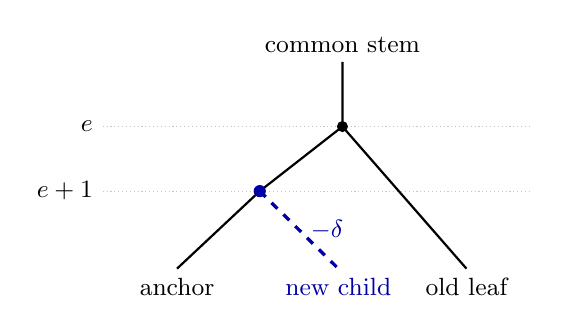
\begin{tikzpicture}[x=1.05cm,y=0.82cm,>=stealth,font=\small]
 \draw[gray!45,densely dotted] (-2.9,-1) -- (2.3,-1);
 \draw[gray!45,densely dotted] (-2.9,-2) -- (2.3,-2);
 \node[left] at (-2.9,-1) {$e$};
 \node[left] at (-2.9,-2) {$e+1$};
 \draw[thick] (0,0) -- (0,-1) -- (-1,-2) -- (-2,-3.2);
 \draw[thick] (0,-1) -- (1.5,-3.2);
 \draw[blue!65!black,very thick,dashed] (-1,-2) -- (-0.05,-3.2);
 \fill (0,-1) circle (2pt);
 \fill[blue!65!black] (-1,-2) circle (2.2pt);
 \node[above] at (0,0) {common stem};
 \node[below] at (-2,-3.2) {anchor};
 \node[below,blue!65!black] at (-0.05,-3.2) {new child};
 \node[below] at (1.5,-3.2) {old leaf};
 \node[right,blue!65!black] at (-0.5,-2.6) {$-\delta$};
\end{tikzpicture}
\caption{One local effect of delaying a target split. The old tree is solid;
the dashed child creates a split at the previously unary depth-$e+1$ vertex,
with coefficient $m_{e+1}-m_{e+2}=-\delta$.
The proof shifts every internal target depth and charges distinct vertices
separately, even when their depths coincide. Later target colors may reuse
eligible old leaves.}
\label{decor:shift-figure}
\end{figure}

Let $\kappa(T)$ be the reference coefficient \eqref{tree:K}, and put
\begin{equation}
 J=\kappa(S^+)^2.
 \label{decor:J-definition}
\end{equation}
At each
vertex the $j=1$ factor is $-\delta$; for $j\ge2$ its absolute value
is at least $\eta/2$ for all sufficiently large $L$.  If $b=b(S)$,
then
\begin{equation}
 |J|\ge c_{k,\eta}\delta^{2b}>0.
 \label{decor:J-lower-bound}
\end{equation}
For large $L$, regularity ensures that each shifted depth differs from
every branching depth of the old tree, including $d$. Thus these $2b$
target branching vertices must be created by fresh unary splits.
Lemma~\ref{tree:charging} gives
\begin{equation}
 \frac1{|J|}\sum_{\text{allowed extensions}}|c|
        \le C_{k,\eta}.
 \label{decor:relative-absolute-cost}
\end{equation}
The two copies have aligned depths but distinct branching vertices:
each vertex supplies its own factor $\delta$. This is the reason for
the shift. The full signed coefficient has an additional factor
$-\delta$ from separation at $d$; we divide by $J$ and leave that
factor in the identity. Equation~\eqref{decor:relative-absolute-cost}
then controls every projection error after division.

\paragraph{Projecting the two target sides.}
In every extension, the marginal target tree consists of two
ordinary copies of $S^+$, independent below their separation at $d$.
By \eqref{decor:projection-bound} its multioverlap differs in
$L^2$ from the contraction of its projected means at $e+1$ by at
most $2p_N(S^+,e+1)$.  Change the proper child depths back by one,
then change their evaluation depth from $e+1$ to $e$.  The product
difference inequality and Lemma~\ref{decor:depth-continuity} show
that this adds an error at most $h_N(S)$ in $L^2$, with
\begin{equation}
 \mathcal A_{L,\eta}h_N(S)^2\le C_k/L.
 \label{decor:projection-shift-error}
\end{equation}
One can take $h_N(S)$ to be the sum of the finitely many
$L^2(\|\cdot\|_N)$ distances in these comparisons, multiplied by
a size-dependent constant.  This definition depends only on the
single-copy marginal shapes, not on the particular extension.
Thus \eqref{decor:projection-shift-error} holds uniformly for the
comparisons in the extension sum, even though the union of the
old and target trees itself need not have regular depths.

Let $a,b$ denote the vectors $a_{S,e}$ on the old stems I and II.
The target stem in I shares the old prefix through $e$ because it
contains the anchor, so its final projected vector is $a$.

\paragraph{The signed extension sum.}
Set $f$ to be the overlap of all $2k$ old leaves, an allowed fixed
overlap monomial. All target-I additions stay in the anchor's branch
below $d$, so they leave the old-II stem and its child counts unchanged.
Classify the first added path of target side II by its prefix
through $e$.  It may diverge freshly at $\ell=d$, with coefficient
$-c_d$, or follow the old II stem and diverge at $d<\ell<e$, with
coefficient $-c_\ell=-\delta$.  In such a class let $b_\ell$ be
$a_{S,e}$ on the new stem; it shares the old II prefix through
$\ell$.  At $\ell=d$ the stems carrying $a,b,b_d$ are conditionally
independent below $d$.  Every remaining possibility follows the
old II prefix through $e$ and has final projected vector $b$.
All later target paths in side II follow its first path through
$e$, since their earliest split is $e+1$.

For a fixed extension history, retain every old path and the first
target-II prefix through $e$, and delete all other new branches.
The target-I projection $a$ already depends only on the retained old
anchor prefix. Each deleted subtree integrates to one under its
probability kernels; a reused old leaf introduces no new variable.
The retained tree depends only on the class: it is the old tree with a
fresh stem attached at $\ell<e$, or just the old tree in the remaining
class. The history is a combinatorial choice, not a condition on sampled
values. Thus the joint marginal of the old paths and projected prefixes
is fixed within each class. In particular, the expectation of $f$ times
the projected overlap is constant within a class and can be multiplied
by its total signed coefficient.

By Lemma~\ref{tree:reference-total}, summing later side-II colors
backwards gives $\kappa(S^+)$ for each first-path choice.  Summing the
side-I choices gives the other factor $\kappa(S^+)$. The fresh class
at $\ell$ therefore has total coefficient $-c_\ell J$.
The total coefficient is $-\delta J$, both from the old tree and
from the anchor alone. Since
\[
 \sum_{\ell=d}^{e-1}c_\ell=(e+1)\delta=m_e+\delta,
\]
the remaining prefix-through-$e$ class has coefficient $m_eJ$.
Thus the projected terms have the following coefficients:
\[
 \begin{array}{c|c|c}
 \text{side-II prefix} & \text{projected overlap}
      & \text{total coefficient}\\ \hline
 \text{fresh divergence at }d\le\ell<e & a\cdot b_\ell & -c_\ell J\\
 \text{old prefix through }e & a\cdot b & m_eJ
 \end{array}
\]

Multiply the projected overlap in each row by $f$ and divide the
prescribed-tree identity by $J$. Rearranging gives
\begin{equation}
 \sum_{\ell=d}^{e-1}c_\ell
   \mathbb E\bigl[f(a\cdot b-a\cdot b_\ell)\bigr]
 =\delta\bigl(\mathbb E[f(a\cdot b)]
          -\mathbb Ef\,\mathbb ER_{\mathrm{target}}\bigr)
       +\rho_N(S,d),
 \label{decor:induction-identity}
\end{equation}
where $R_{\mathrm{target}}$ on the right is the target overlap in
the anchor-alone extension.  Its absolute value is at most one.
The error satisfies
\begin{equation}
 |\rho_N(S,d)|\le C_{k,\eta}
       \bigl(p_N(S^+,e+1)+h_N(S)\bigr)
       +C_{L,k,\eta}\varepsilon_{N,L,k}.
 \label{decor:induction-error}
\end{equation}
Indeed, multiplying a projection error by $f$, even when correlated
with it, costs at most its $L^2$ norm since $|f|\le1$. Sum these errors
with absolute coefficients and apply
\eqref{decor:relative-absolute-cost}. The final term includes division
of the original identity error by $J$ and tends to zero at fixed $L$.

\paragraph{Closing the induction.}
Equation~\eqref{decor:projection-bound} gives
$\|f-a\cdot b\|_{L^2}\le2p_N(S,e)$.
Moreover
$\sum_{\ell=d}^{e-1}c_\ell=(e+1)\delta\le1$.
Replacing $f$ by $a\cdot b$ on the left of
\eqref{decor:induction-identity} therefore costs at most
$4p_N(S,e)$.  Each $a\cdot b_\ell$ has the same marginal law as
$a\cdot b$, so that left side becomes
\[
 \frac12\sum_{\ell=d}^{e-1}c_\ell
        \mathbb E(a\cdot b-a\cdot b_\ell)^2.
\]
Its summands are nonnegative and $c_d\ge\eta$.  The right side
of \eqref{decor:induction-identity} is bounded in absolute value
by $2\delta+|\rho_N(S,d)|$.  Hence
\begin{equation}
 \mathbb E(a\cdot b-a\cdot b_d)^2
 \le C_\eta\bigl(\delta+p_N(S,e)+|\rho_N(S,d)|\bigr).
 \label{decor:projected-three-copy}
\end{equation}
Sample three copies of $A_S$ conditionally independently below
$d$.  Projecting each of the two contractions involving the
first copy changes it in $L^2$ by at most $2p_N(S,e)$.
Using \eqref{decor:three-copy-bound},
\eqref{decor:projected-three-copy}, and $p_N(S,e)\le k$, we obtain
\begin{equation}
 v_N(S,d)\le C_{k,\eta}\bigl(
       \delta+p_N(S,e)+p_N(S^+,e+1)+h_N(S)\bigr)
       +C_{L,k,\eta}\varepsilon_{N,L,k}.
 \label{decor:covariance-induction-estimate}
\end{equation}
Each child in either $p_N$ has fewer than $k$ leaves. To make the
averaging step explicit, the aligned construction has
$D=b(S)+1$ distinct depth coordinates, including $d$ and $e$.
A term belonging to $T_j$ uses only $D_j=b(T_j)+1$ coordinates.
For the shifted term these are
$\pi_j(\mathbf q)=(e+1,(q_v+1)_{v\in\operatorname{Br}(T_j)})$.
Every retained assignment has at most $L^{D-D_j}$ preimages, and its
coordinates are $\eta/2$-regular for large $L$. If $w_j$ is the child
covariance as a function of these coordinates, then, for $0<\gamma\le1$,
\begin{align}
 L^{-D}\sum_{\mathbf q\;\eta\text{-regular}}
       w_j(\pi_j(\mathbf q))^\gamma
 &\le L^{-D_j}\sum_{\mathbf y\;\eta/2\text{-regular}}w_j(\mathbf y)^\gamma
 \notag\\
 &\le\left(L^{-D_j}\sum_{\mathbf y\;\eta/2\text{-regular}}
       w_j(\mathbf y)\right)^\gamma.
 \label{decor:fiber-bound}
\end{align}
The unshifted term has the same bound without translating the coordinates.
Thus the two aligned copies use single-copy estimates; there is no
restriction of an independently averaged pair of copies to a diagonal.
Taking $\gamma=1/4$ and then $\limsup_N$, and using
\eqref{decor:projection-shift-error} and
\eqref{decor:identity-error}, gives, for sufficiently large $L$,
\begin{equation}
 V_{k,L}(\eta)\le C_{k,\eta}\left(
       L^{-1/2}+V_{k-1,L}(\eta/2)^{1/4}\right).
 \label{decor:induction-recursion}
\end{equation}
The maximum over smaller topologies in \eqref{decor:V-definition}
can be absorbed in the right side because these covariances are
bounded by one.  The base case and induction now imply
$V_{k,L}(\eta)\to0$ for every fixed $k,\eta$, proving the proposition.
\end{proof}

\subsection{Concentration of every multioverlap}

The covariance estimate controls fluctuations below a sampled prefix.
We now use a marker anchor to concentrate the prefix projection, and
combine this with the averaged continuity estimate.

\begin{proof}[Proof of \cref{decor:overlap-concentration}]
For a singleton, use the spin-anchor identity with no added colors
and $f=R_S$.  It gives
$\mathbb ER_S^2=(\mathbb ER_S)^2+o_N(1)$.

Suppose $S$ first splits at $e$ and has proper child shapes
$T_1,\ldots,T_s$. We will condition one step before $e$. Use $S$ as
the old tree, designate one of its
leaves as a marker anchor, and add a full copy of $S$ all of whose
leaves split from the anchor at $e-1$.  Its first path must be
fresh at $e-1$, because the old tree has not yet branched there.
All other target paths lie in the resulting fresh subtree.
The extension coefficient on both sides of the prescribed-tree
identity is the same nonzero number
\begin{equation}
 C(S,e)=-\delta \kappa(S).
 \label{decor:marker-coefficient}
\end{equation}
The target and old copies are conditionally independent and
identically distributed below $\mathscr F_{e-1}$. With
$f=R_S$ and $M=\mathbb E[R_S\mid\mathscr F_{e-1}]$, their product has
conditional expectation $M^2$. On the anchor-alone side, deleting the
marker's continuation below $e-1$ integrates a probability kernel to one
and leaves the ordinary target law $S$, with mean $\mathbb E R_S$.
The identity therefore gives
\begin{equation}
 C(S,e)\bigl(\mathbb EM^2-(\mathbb E R_S)^2\bigr)
 =C(S,e)\operatorname{Var}(M)=o_N(1),
 \label{decor:marker-variance-identity}
\end{equation}
and hence
\begin{equation}
 \qquad \operatorname{Var}(M)\longrightarrow0
 \quad\text{at each fixed }L,S,e.
 \label{decor:prefix-projection-concentration}
\end{equation}
Division by $C(S,e)$ is made only at fixed $L$; no uniform lower
bound as $L\to\infty$ is needed.

It remains to control the conditional variance below this prefix.
The child covariances are evaluated at $e$, which is separated from
all their branching depths; the move to $e-1$ will use martingale
continuity instead. Set
\[
 G=\mathbf1\cdot\prod_j \mu_{e,T_j},
 \qquad G_-=\mathbf1\cdot\prod_j \mu_{e-1,T_j}.
\]
The latter is $\mathscr F_{e-1}$-measurable.  By
\eqref{decor:projection-bound},
$\mathbb E(R_S-G)^2\le p_N(S,e)^2$.
Keeping all proper child depths fixed, the product difference
inequality and \eqref{decor:martingale-energy} imply
\begin{equation}
 \mathcal A_{L,\eta}\mathbb E(G-G_-)^2\le C_k/L.
 \label{decor:adjacent-prefix-error}
\end{equation}
Here $e$ is itself a ranged coordinate, so the one-step increments
are summed before division by $L$.  Since conditional expectation
is the optimal $L^2$ projection,
\[
 \mathbb E(R_S-M)^2
   \le\mathbb E(R_S-G_-)^2
   \le2p_N(S,e)^2+2\mathbb E(G-G_-)^2.
\]
Variance decomposition and
\eqref{decor:prefix-projection-concentration} now show
\begin{equation}
 \limsup_{N\to\infty}
      \mathcal A_{L,\eta}\operatorname{Var}(R_S)
 \le C_k\left(L^{-1}+V_{k-1,L}(\eta/2)^{1/2}\right)
 \quad\text{for all sufficiently large }L.
 \label{decor:variance-estimate}
\end{equation}
In this estimate we used
$p_N(S,e)^2\le s\sum_jv_N(T_j,e)^{1/2}$ and
\eqref{decor:fiber-bound} with $\gamma=1/2$: here the full average has
$D=b(S)$ coordinates because $d$ is absent, while still
$D_j=b(T_j)+1$. Proposition~\ref{decor:conditional-concentration}
finishes the proof.
\end{proof}

\begin{remark}
\label{decor:order-of-limits}
All uncancelled small denominators in this section occur only in prescribed-tree
identity errors.  At fixed $L$ there are finitely many relevant trees,
so those errors disappear before any depth average or $L$ limit is
taken.  Errors that survive the $N$ limit are controlled by the
uniform relative absolute-cost bound
\eqref{decor:relative-absolute-cost}, the lower-order covariance
averages, and the martingale estimate $C/L$.  No rate of convergence
in $N$ uniform in $L$ is used.
\end{remark}

\section{Independent hierarchical messages and the cavity comparison}
\label{comp:section}

We turn the reservoir into a trial law in three steps: encode its full
one-site branching law, use multioverlap concentration to separate the
sites, and compare the resulting insertion logarithms.

Fix $\eps>0$. At each depth $L\ge2$, use the sequence of sizes and
deterministic parameter choices supplied by \cref{pert:selection}.
Write $N$ for sizes on this sequence. The choices may depend on $L$, and all statements below concern
these choices. Retain $\underline F$ for the liminf over \emph{all} system
sizes of the bounded model, as before selection. In particular,
\begin{equation}\label{comp:low-increments}
 \Delta_N^{L,\mathbf u_{L,N}}\le\underline F+2\eps.
\end{equation}

\subsection{Encoding a single-site tree}

\begin{lemma}[Recursive law encoding]\label[lemma]{comp:encoding}
For each fixed $N$, $L\ge2$, and selected parameter vector, with the reservoir
root disorder averaged, there is a deterministic trial law
$\zeta_{L,N}\in\mathcal M_L$ whose single-label spin process has the same
expected spin products on every prescribed tree as a uniformly chosen site
of the reservoir. Different trial labels can be chosen independently.
\end{lemma}

\begin{proof}
Include an independent uniform site $i\in[N]$ in the root variable, along
with the reservoir root disorder. Sample the tilted reservoir auxiliary
kernels along each path, and let $\mathscr G_d$ be the sigma-field generated
by this enlarged root and the full auxiliary prefix through depth $d$.
At depth $r=L-1$ put
\[
 x=\arctanh\angles{\sigma_i},
\]
where the brackets denote the leaf Gibbs expectation. This is finite:
at finite $N$ all configuration weights are strictly positive, so
$-1<\angles{\sigma_i}<1$.
Thus $x$ is determined at depth $r$, before the terminal spin transition
at depth $L$. At each terminal replica leaf, draw a spin with law $q_x$. Given the
auxiliary prefix, these spins are independent and have exactly the
one-site law of the independent terminal Gibbs replicas.

Define the random measures backward by
\[
 \eta_{r-1}=\operatorname{Law}(x\mid\mathscr G_{r-1}),\qquad
 \eta_d=\operatorname{Law}(\eta_{d+1}\mid\mathscr G_d)
 \quad(0\le d<r-1).
\]
Then $\eta_d\in\mathcal M_{r-d}$, so
$\zeta_{L,N}=\operatorname{Law}(\eta_0)\in\mathcal M_L$.
All state spaces are standard
Borel, so these conditional probability kernels have measurable versions.
The auxiliary priors used here may be taken to be finite products of finite
mark spaces at each realized root; hence the same assertion also follows
directly by finite sums conditional on the root counts.

Here is an explicit verification for every branching pattern. Fix a
descendant tree $T$ and prescribe a spin $e_a$ at each terminal leaf.
At depth $r$, its conditional probability is
$G_T(x)=\prod_a q_x(e_a)$. At depth $d<r$, let $T_1,\ldots,T_j$ be
the subtrees rooted at its children. Conditional independence of children
gives the backward recursion
\[
 G_T(\eta_d)=\prod_{\ell=1}^j
       \int G_{T_\ell}(\nu)\,\eta_d(d\nu).
\]
By induction, this probability depends on the full prefix only through
$\eta_d$. Thus the nested measures preserve the joint output law of every
descendant tree, including unary stretches and arbitrary numbers of
children. This recursion is precisely the branching version of
\eqref{model:chain}. Taking $\zeta_{L,N}=\operatorname{Law}(\eta_0)$
preserves the root mixture as well. In particular, for every subset $S$
of the leaves,
\begin{equation}\label{comp:single-label-moments}
 \E\prod_{a\in S}\tau^a
 =\frac1N\sum_{i=1}^N\E\prod_{a\in S}\sigma_i^a
 =\E R_S.
\end{equation}
Use independent copies of the entire construction, including the reservoir
root and uniform site, for different labels. The resulting messages are
independent of the new physical disorder in the cavity insertions.
\end{proof}

\subsection{From multioverlaps to spin patterns}

\begin{lemma}[Empirical-pattern comparison]\label[lemma]{comp:patterns}
Fix a prescribed tree with $k$ leaves. Suppose an observable of absolute
value at most one uses the replica-spin patterns at $a$ independent uniform
site labels. Replacing these patterns by $a$ independent trial-label patterns
from \cref{comp:encoding} changes its expected value by at most
\begin{equation}\label{comp:pattern-error}
 a\sum_{\varnothing\ne S\subseteq[k]}\E|R_S-\E R_S|.
\end{equation}
The observable may also depend on new insertion disorder, independent of
the reservoir.
\end{lemma}

\begin{proof}
Conditional on the sampled reservoir configurations, the pattern
$\boldsymbol\sigma_i=(\sigma_i^1,\ldots,\sigma_i^k)$ at a uniform site
has empirical distribution
\[
 \pi(\boldsymbol e)=\frac1N\sum_i
 \prod_{b=1}^k\frac{1+e_b\sigma_i^b}{2}
 =2^{-k}\sum_{S\subseteq[k]}R_S\prod_{b\in S}e_b,
 \qquad \boldsymbol e\in\{-1,1\}^k.
\]
The trial-label distribution is $\bar\pi=\E\pi$ by
\eqref{comp:single-label-moments}. Independent uniform sampling with
replacement gives $\pi^{\otimes a}$ conditionally in the reservoir; the
trial distribution is $\bar\pi^{\otimes a}$. The elementary telescoping
bound for product measures gives
\[
 \norm{\pi^{\otimes a}-\bar\pi^{\otimes a}}_{\rm TV}
 \le a\norm{\pi-\bar\pi}_{\rm TV}
 \le\frac a2\sum_{\varnothing\ne S\subseteq[k]}|R_S-\E R_S|.
\]
Integrating a function bounded by one costs at most twice total variation.
Conditioning on the independent insertion disorder proves the last assertion.
\end{proof}

Let $Q_k$ be the tree law in \cref{tree:log-expansion}. We need the following
consequence of the decorrelation theorem:
\begin{equation}\label{comp:shape-error}
 \lim_{L\to\infty}\limsup_{N\to\infty}
 \E_{Q_k}\sum_{\varnothing\ne S\subseteq[k]}
 \E|R_S-\E R_S|=0\qquad(k\text{ fixed}).
\end{equation}
Here and below the inner limit is along the selected fixed-$L$ sequence.
To see this, fix $0<\eta<1/2$, and let $\mathfrak S_k$ be the finite collection
of labeled topologies on nonempty subsets of $[k]$. We claim the bound
\begin{equation}\label{comp:shape-error-bound}
 \E_{Q_k}\sum_{\varnothing\ne S\subseteq[k]}
       \E|R_S-\E R_S|
 \le C_k\left(\eta+L^{-1}
       +\sum_{U\in\mathfrak S_k}
          \bigl(\mathcal A_{L,\eta}\Var(R_U)\bigr)^{1/2}\right).
\end{equation}
The average for a singleton has no depth coordinates.
By \cref{tree:regular-shapes}, nonregular trees
have probability at most $C_k(\eta+L^{-1})$. On regular trees every induced
subtree retains the interior and separation conditions on its branching
depths. For a topology with $a$ branching vertices, each depth assignment
has probability at most $C_kL^{-a}$. If an induced subtree retains $a'$
branching vertices, each assignment of its depths has at most $L^{a-a'}$
extensions to the full tree. Summing out these unused coordinates leaves
exactly the normalization $L^{-a'}$ in $\mathcal A_{L,\eta}$.
Cauchy--Schwarz bounds the resulting average of mean absolute deviations
by $\bigl(\mathcal A_{L,\eta}\Var(R_U)\bigr)^{1/2}$.
Summing over the finitely many topologies and subsets, and using the bound
two for each deviation on nonregular trees, proves
\eqref{comp:shape-error-bound}. Apply \cref{decor:overlap-concentration}
first at fixed $\eta$, taking the fixed-$L$ limit in $N$ before
$L\to\infty$, and then let $\eta\downarrow0$ to obtain
\eqref{comp:shape-error}.

\subsection{Comparison of the insertion logarithms}

\begin{proposition}\label[proposition]{comp:insertion-comparison}
For the trial laws of \cref{comp:encoding}, with
$\mathbf m^{(L)}=(1/L,\ldots,(L-1)/L)$,
\begin{equation}\label{comp:increment-comparison}
 \lim_{L\to\infty}\limsup_{N\to\infty}
 \left|\Delta_N^{L,\mathbf u_{L,N}}
 -\cB_{L-1}(\zeta_{L,N},\mathbf m^{(L)})\right|=0.
\end{equation}
\end{proposition}

\begin{proof}
For each insertion in \cref{cavity:increment}, replace the reservoir spins
at its site labels by independent spin processes from \cref{comp:encoding}.
Denote the resulting trial insertions by $\widetilde A_{\rm s}$ and
$\widetilde A_{\rm b}$, and their recursions from
\eqref{tree:Y-recursion} by $\widetilde Y_{0,\rm s}$ and
$\widetilde Y_{0,\rm b}$. These recursions use the trial kernels.

At the terminal spin transition, averaging $\widetilde A_{\rm s}$ over
its independent trial spins gives exactly $V_{\rm s}$ in
\eqref{model:vs}; hence $\widetilde Y_{0,\rm s}=T_0V_{\rm s}$.
For $\widetilde A_{\rm b}$ the same transition gives a product of
$K_{\rm b}$ edge factors with disjoint message labels. Given the physical
disorder and all message prefixes at a depth, these label groups remain
independent. Their product therefore factors through each conditional
power mean, successively from the last level to the first. Consequently,
\[
 \begin{aligned}
 \E\log\widetilde Y_{0,\rm b}
 &=\alpha(p-1)\E\log T_0V_{\rm e},\\
 \log2+\E\log\widetilde Y_{0,\rm s}
       -\E\log\widetilde Y_{0,\rm b}
 &=\cB_{L-1}(\zeta_{L,N},\mathbf m^{(L)}).
 \end{aligned}
\]
By \eqref{cavity:identity}, it remains to compare the reservoir and trial
insertion logarithms in the stated limits.

Consider either insertion and first restrict its
Poisson count $K$ to $K\le M$, where $M$ is fixed. Set
$C=H+BM$, $z=\cosh C$, and $c=\tanh C<1$. On this event both the reservoir
insertion and its trial version can be written as
$A=z(1+D)$ with $|D|\le c$, uniformly in all disorder and path variables.
The deterministic term $\log z$ cancels in the comparison.

At each order $k$ of \cref{tree:log-expansion}, the product of the $k$
copies of $D$ is a bounded function of replica-spin patterns at at most
$pM$ labels and of independent insertion disorder. By
\cref{comp:patterns}, its evaluation error on a fixed tree is bounded by
$pM\sum_{S\ne\varnothing}\E|R_S-\E R_S|$. Hence
\eqref{comp:shape-error} makes its tree-averaged error tend to zero in the
ordered limits. For every fixed $M$, truncating the expansion after $q$
terms leaves an error at most
$\sum_{k>q}c^k/k$ on either side, uniformly in $N,L$.

Outside the count cutoff the original insertion logarithms, on both sides,
are bounded by $H+BK$. Their expected contribution is therefore at most
$2\E[(H+BK)\mathbf1_{\{K>M\}}]$, which tends to zero as $M\to\infty$.
This proves convergence of the expected insertion logarithms: explicitly,
first choose $M$ to control the Poisson tail, then $q$ to control the
geometric tail, and then take the limits in $N$ and $L$ for the finitely
many remaining expansion terms. Together with the trial identities above
and \eqref{cavity:identity}, this proves \eqref{comp:increment-comparison}.
\end{proof}

\begin{corollary}\label[corollary]{comp:bounded-lower}
For every bounded permutation-invariant interaction law and bounded field
law, with the functionals defined in \cref{model:section},
\[
 \liminf_{N\to\infty}F_N\ge\inf_{r\ge0}\Phi_r.
\]
\end{corollary}

\begin{proof}
Write $A=\inf_{r\ge0}\Phi_r$, which is finite by
\eqref{model:trial-bounds}. Each encoded trial value is at least $A$, so
\eqref{comp:low-increments} gives, at every fixed $L$,
\[
 A\le\underline F+2\eps+
 \limsup_{N\to\infty}
 \left|\Delta_N^{L,\mathbf u_{L,N}}
       -\cB_{L-1}(\zeta_{L,N},\mathbf m^{(L)})\right|.
\]
The inner limit uses that depth's selected sequence. Letting $L\to\infty$
in \cref{comp:insertion-comparison} gives
$A\le\underline F+2\eps$, and then $\eps\downarrow0$ proves the result.
\end{proof}

\section{Normalization, truncation, and completion of the proof}
\label{reduction:section}

The lower bound proved in \cref{comp:bounded-lower} requires bounded
permutation-invariant interactions, whereas the upper bound uses the
factorization and positivity hypotheses. An integrable constant shift
and uniform approximation connect the two statements.

\begin{lemma}[Stability]\label{reduction:stability}
Couple two interaction laws $\theta,\theta'$ and two field laws $h,h'$,
each satisfying \eqref{model:integrability} for the fixed $p$ and $\alpha$,
and put $D=\E\max_s|\theta(s)-\theta'(s)|$ and
$d=\E|h-h'|$. Then
\begin{align}
 |F_N-F_N'|&\le\alpha D+d,\label{reduction:free-stability}\\
 |\cB_r(\zeta,\mathbf m)-\cB_r'(\zeta,\mathbf m)|
 &\le\alpha(2p-1)D+d\label{reduction:trial-stability}
\end{align}
uniformly in $N,r$ and all trial laws, including $r=0$.
If $c$ is an integrable random constant associated with an interaction and
$\widehat\theta=\theta-c$, then
\begin{equation}\label{reduction:shift}
 \widehat F_N=F_N-\alpha\E c,
 \qquad\widehat{\cB}_r=\cB_r-\alpha\E c.
\end{equation}
\end{lemma}

\begin{proof}
Use the same counts and indices in the two Hamiltonians. Their pointwise
log-weight difference is bounded by the sum of the interaction sup-norm
differences and field differences. The logarithm of the partition function
preserves this bound, which gives \eqref{reduction:free-stability}.
Each cavity interaction changes by at most the corresponding sup-norm
interaction difference, and so does each edge logarithm. The power means
preserve these root-measurable bounds. The site term has mean $\alpha p$
interactions and the edge term has coefficient $\alpha(p-1)$, giving
\eqref{reduction:trial-stability}.

For \eqref{reduction:shift}, the physical constants factor out of the spin
partition function and of every power mean. In the functional, the site
term shifts by $-\alpha p\E c$ and the edge term contributes
$+\alpha(p-1)\E c$, for a net shift $-\alpha\E c$.
\end{proof}

\begin{proof}[Proof of \cref{main:theorem}]
The multiplier $a$ may depend asymmetrically on the labeled input functions,
so the original interaction law need not be permutation invariant.
We first remove this multiplier by an integrable scalar shift.
Set $c=\theta(1,\ldots,1)$ and $\widehat\theta=\theta-c$. The
constant is integrable, since $|c|\le B(\theta)$. The factorization gives
\[
 \widehat\theta(s)=
 \log\frac{1+b\prod_{\ell=1}^p f_\ell(s_\ell)}
 {1+b\prod_{\ell=1}^p f_\ell(1)}.
\]
The multiplier $a$ has disappeared. Independence and identical distribution
of the $f_\ell$, and their independence of $b$, show that the law of
$\widehat\theta$ is invariant under permutations of its inputs.
Moreover $\E B(\widehat\theta)\le2\E B(\theta)<\infty$.

For $K>0$, truncate each entry of $\widehat\theta$ to $[-K,K]$ and truncate
$h$ to $[-K,K]$, obtaining $\widehat\theta^{(K)},h^{(K)}$.
Permutation invariance is preserved. The bounded-law lower bound
\cref{comp:bounded-lower} applies whether or not truncation preserves the
factorization. By dominated convergence,
\[
 D_K=\E\max_s|\widehat\theta(s)-\widehat\theta^{(K)}(s)|\longrightarrow0,
 \qquad d_K=\E|h-h^{(K)}|\longrightarrow0.
\]
Write $\widehat I$ for the infimum of the normalized trial functional
over all depths and trial laws, and $I_K$ for the same infimum with
the truncated physical laws. The uniform trial estimate gives
\[
 |\widehat I-I_K|\le\alpha(2p-1)D_K+d_K.
\]
The pressure estimate and \cref{comp:bounded-lower} now imply
\[
 \liminf_N\widehat F_N
 \ge I_K-\alpha D_K-d_K
 \ge\widehat I-2\alpha pD_K-2d_K.
\]
Letting $K\to\infty$ proves
$\liminf_N\widehat F_N\ge\widehat I=\inf_r\widehat\Phi_r$.
Undoing the constant shift gives $\liminf_NF_N\ge\inf_r\Phi_r$.
Finally \cref{upper:bound} gives $\limsup_NF_N\le\inf_r\Phi_r$.
Both limits agree, proving existence and \eqref{main:formula}.
\end{proof}

\section{Named models and the zero-temperature limit}
\label{models:section}

The standard examples of the factorization are the diluted spin models
and random satisfiability models of
Franz--Leone and Panchenko--Talagrand~\cite{FL03,PT04}.
We retain the Poisson counts and sampling with replacement specified
in \eqref{model:hamiltonian}.

\begin{corollary}[Viana--Bray and diluted even-spin models]
\label[corollary]{models:spin}
Fix an even integer $p\ge2$, $\alpha>0$, and independent real random
variables $J,H$ such that $J$ has a symmetric distribution and
$\E|J|+\E|H|<\infty$. For every $\beta>0$, the model with
\[
 \theta_\beta(s_1,\ldots,s_p)=\beta J\prod_{\ell=1}^p s_\ell,
 \qquad h_\beta=\beta H
\]
satisfies the variational formula \eqref{main:formula}, with the trial
functional evaluated at these interaction and field laws. In particular,
this holds for the Viana--Bray model~\cite{VB85}, which is the case $p=2$.
\end{corollary}

\begin{proof}
Use
\[
 a=\cosh(\beta J),\qquad b=\tanh(\beta J),\qquad f_\ell(s)=s.
\]
The functions $f_\ell$ are deterministic independent copies, and
$|b|<1$ almost surely. Symmetry makes every odd moment of $b$ zero;
the even moments are nonnegative. Finally,
$B(\theta_\beta)=\beta|J|$ and $|h_\beta|=\beta|H|$.
Thus all hypotheses of \cref{main:theorem} hold.
\end{proof}

\begin{corollary}[Soft random even-$K$ SAT]
\label[corollary]{models:sat}
Fix an even integer $K\ge2$ and $\alpha>0$. Let
$\varepsilon_1,\ldots,\varepsilon_K$ be independent fair signs and let
$W\ge0$ be independent of the signs, with $\E W<\infty$. For every
$\beta>0$, the interaction
\[
 \theta_\beta(s_1,\ldots,s_K)
 =-\beta W\prod_{\ell=1}^K\frac{1+\varepsilon_\ell s_\ell}{2},
 \qquad h=0,
\]
satisfies \eqref{main:formula}. The choice $W=1$ is the soft random
even-$K$ SAT model; $W$ gives an independent nonnegative clause weight.
\end{corollary}

\begin{proof}
The product
$I_\varepsilon(s)=\prod_\ell(1+\varepsilon_\ell s_\ell)/2$ takes
values in $\{0,1\}$ and indicates a violated clause. Therefore
\[
 e^{\theta_\beta(s)}
 =1+(e^{-\beta W}-1)I_\varepsilon(s).
\]
Take $a=1$, $b=e^{-\beta W}-1$, and
$f_\ell(s)=(1+\varepsilon_\ell s)/2$. The functions are independent
copies and independent of $b$. Since $0\le-b<1$, the strict product
condition and every positivity inequality hold. Moreover,
$B(\theta_\beta)=\beta W$, so \cref{main:theorem} applies.
\end{proof}

For the spin model, define the unscaled energy score by
\[
 \mathcal E_N(\sigma)
 =\sum_{k=1}^{M_N}J_k\prod_{\ell=1}^p\sigma_{i_{\ell,k}}
   +\sum_{i=1}^N H_i\sigma_i.
\]
For the satisfiability model, put
\[
 \mathcal E_N(\sigma)
 =-\sum_{k=1}^{M_N}W_k
      \prod_{\ell=1}^K\frac{1+\varepsilon_{\ell,k}
       \sigma_{i_{\ell,k}}}{2}.
\]
These scores and their disorder laws do not depend on $\beta$; in
both cases the partition function is
$Z_N(\beta)=\sum_\sigma e^{\beta\mathcal E_N(\sigma)}$.
Let $\cB_{r,\beta}$ denote the functional
\eqref{model:functional} for the corresponding laws at inverse
temperature $\beta$.

\begin{corollary}[Zero-temperature variational limit]
\label{models:ground}
For each model in \cref{models:spin,models:sat}, the limit
\[
 g=\lim_{N\to\infty}\frac1N\E\max_\sigma\mathcal E_N(\sigma)
\]
exists and satisfies
\begin{equation}\label{models:ground-formula}
 g=\lim_{\beta\to\infty}\frac1\beta
       \inf_{r\ge0}\inf_{\zeta,\mathbf m}
          \cB_{r,\beta}(\zeta,\mathbf m).
\end{equation}
More precisely, the expression inside the temperature limit lies in
$[g,g+\log(2)/\beta]$. For unit-weight SAT, the limiting expected
minimum number of violated clauses per variable is $-g$.
\end{corollary}

\begin{proof}
Write $g_N=N^{-1}\E\max_\sigma\mathcal E_N(\sigma)$ and
$P_N(\beta)=N^{-1}\E\log Z_N(\beta)$. The first-moment assumptions
make $g_N$ finite and uniformly bounded. Since there are $2^N$ spin
configurations,
\[
 g_N\le\frac{P_N(\beta)}\beta
       \le g_N+\frac{\log2}{\beta}.
\]
For each fixed $\beta>0$, \cref{main:theorem} gives
$P_N(\beta)\to I(\beta)$, where
$I(\beta)=\inf_{r,\zeta,\mathbf m}\cB_{r,\beta}(\zeta,\mathbf m)$.
Hence
\[
 \limsup_N g_N\le\frac{I(\beta)}\beta
   \le\liminf_N g_N+\frac{\log2}{\beta}.
\]
Letting $\beta\to\infty$ proves that $g_N$ converges to a limit $g$.
Taking $N\to\infty$ in the finite-volume bounds now gives
$g\le I(\beta)/\beta\le g+\log(2)/\beta$, proving
\eqref{models:ground-formula}. In the satisfiability model, maximizing
the negative violation count is the same as minimizing that count.
\end{proof}

The infimum in \eqref{models:ground-formula} is taken over all finite
hierarchies separately at each positive temperature. The formula
does not require attainment or a limiting hierarchy.

\begin{remark}
The even-arity hypothesis in \cref{models:sat} excludes random 3-SAT.
For that model, the companion~\cite[Theorem~8.4]{OpenAIThreeSAT2026}
gives an exact soft-pressure formula over finite rational trials for a
Poisson number of clauses whose variable positions are sampled independently
with replacement. Its sign-indexed message pairs need not form a probability
distribution, and its trial functional differs from \eqref{model:functional}.
\end{remark}

\bibliographystyle{plain}
\bibliography{references}
\end{document}
